\documentclass[twoside]{book}

% Packages required by doxygen
\usepackage{calc}
\usepackage{doxygen}
\usepackage{graphicx}
\usepackage[utf8]{inputenc}
\usepackage{makeidx}
\usepackage{multicol}
\usepackage{multirow}
\usepackage{textcomp}
\usepackage[table]{xcolor}

% Font selection
\usepackage[T1]{fontenc}
\usepackage{mathptmx}
\usepackage[scaled=.90]{helvet}
\usepackage{courier}
\usepackage{amssymb}
\usepackage{sectsty}
\renewcommand{\familydefault}{\sfdefault}
\allsectionsfont{%
  \fontseries{bc}\selectfont%
  \color{darkgray}%
}
\renewcommand{\DoxyLabelFont}{%
  \fontseries{bc}\selectfont%
  \color{darkgray}%
}

% Page & text layout
\usepackage{geometry}
\geometry{%
  a4paper,%
  top=2.5cm,%
  bottom=2.5cm,%
  left=2.5cm,%
  right=2.5cm%
}
\tolerance=750
\hfuzz=15pt
\hbadness=750
\setlength{\emergencystretch}{15pt}
\setlength{\parindent}{0cm}
\setlength{\parskip}{0.2cm}
\makeatletter
\renewcommand{\paragraph}{%
  \@startsection{paragraph}{4}{0ex}{-1.0ex}{1.0ex}{%
    \normalfont\normalsize\bfseries\SS@parafont%
  }%
}
\renewcommand{\subparagraph}{%
  \@startsection{subparagraph}{5}{0ex}{-1.0ex}{1.0ex}{%
    \normalfont\normalsize\bfseries\SS@subparafont%
  }%
}
\makeatother

% Headers & footers
\usepackage{fancyhdr}
\pagestyle{fancyplain}
\fancyhead[LE]{\fancyplain{}{\bfseries\thepage}}
\fancyhead[CE]{\fancyplain{}{}}
\fancyhead[RE]{\fancyplain{}{\bfseries\leftmark}}
\fancyhead[LO]{\fancyplain{}{\bfseries\rightmark}}
\fancyhead[CO]{\fancyplain{}{}}
\fancyhead[RO]{\fancyplain{}{\bfseries\thepage}}
\fancyfoot[LE]{\fancyplain{}{}}
\fancyfoot[CE]{\fancyplain{}{}}
\fancyfoot[RE]{\fancyplain{}{\bfseries\scriptsize Generated on Mon Apr 25 2016 03\-:02\-:18 for Nysse\-Osu by Doxygen }}
\fancyfoot[LO]{\fancyplain{}{\bfseries\scriptsize Generated on Mon Apr 25 2016 03\-:02\-:18 for Nysse\-Osu by Doxygen }}
\fancyfoot[CO]{\fancyplain{}{}}
\fancyfoot[RO]{\fancyplain{}{}}
\renewcommand{\footrulewidth}{0.4pt}
\renewcommand{\chaptermark}[1]{%
  \markboth{#1}{}%
}
\renewcommand{\sectionmark}[1]{%
  \markright{\thesection\ #1}%
}

% Indices & bibliography
\usepackage{natbib}
\usepackage[titles]{tocloft}
\setcounter{tocdepth}{3}
\setcounter{secnumdepth}{5}
\makeindex

% Hyperlinks (required, but should be loaded last)
\usepackage{ifpdf}
\ifpdf
  \usepackage[pdftex,pagebackref=true]{hyperref}
\else
  \usepackage[ps2pdf,pagebackref=true]{hyperref}
\fi
\hypersetup{%
  colorlinks=true,%
  linkcolor=blue,%
  citecolor=blue,%
  unicode%
}

% Custom commands
\newcommand{\clearemptydoublepage}{%
  \newpage{\pagestyle{empty}\cleardoublepage}%
}


%===== C O N T E N T S =====

\begin{document}

% Titlepage & ToC
\hypersetup{pageanchor=false}
\pagenumbering{roman}
\begin{titlepage}
\vspace*{7cm}
\begin{center}%
{\Large Nysse\-Osu }\\
\vspace*{1cm}
{\large Generated by Doxygen 1.8.5}\\
\vspace*{0.5cm}
{\small Mon Apr 25 2016 03:02:18}\\
\end{center}
\end{titlepage}
\clearemptydoublepage
\tableofcontents
\clearemptydoublepage
\pagenumbering{arabic}
\hypersetup{pageanchor=true}

%--- Begin generated contents ---
\chapter{Hierarchical Index}
\section{Class Hierarchy}
This inheritance list is sorted roughly, but not completely, alphabetically\-:\begin{DoxyCompactList}
\item Kaupunki\-R\-P\begin{DoxyCompactList}
\item \contentsline{section}{Kaupunki}{\pageref{class_kaupunki}}{}
\end{DoxyCompactList}
\item Matkustaja\begin{DoxyCompactList}
\item \contentsline{section}{Aly\-Matkustaja}{\pageref{class_aly_matkustaja}}{}
\end{DoxyCompactList}
\item Q\-Dialog\begin{DoxyCompactList}
\item \contentsline{section}{Lopetus\-Dialog}{\pageref{class_lopetus_dialog}}{}
\end{DoxyCompactList}
\item Q\-Graphics\-Item\begin{DoxyCompactList}
\item \contentsline{section}{Nyssekuva}{\pageref{class_nyssekuva}}{}
\end{DoxyCompactList}
\item Q\-Graphics\-Object\begin{DoxyCompactList}
\item \contentsline{section}{Ammus}{\pageref{class_ammus}}{}
\begin{DoxyCompactList}
\item \contentsline{section}{Laser}{\pageref{class_laser}}{}
\item \contentsline{section}{Miina}{\pageref{class_miina}}{}
\item \contentsline{section}{Rynnakkokivaari}{\pageref{class_rynnakkokivaari}}{}
\end{DoxyCompactList}
\item \contentsline{section}{Drooni}{\pageref{class_drooni}}{}
\end{DoxyCompactList}
\item Q\-Graphics\-Scene\begin{DoxyCompactList}
\item \contentsline{section}{Peli\-Alue}{\pageref{class_peli_alue}}{}
\end{DoxyCompactList}
\item Q\-Object\begin{DoxyCompactList}
\item \contentsline{section}{Kaupunki}{\pageref{class_kaupunki}}{}
\end{DoxyCompactList}
\item Q\-Widget\begin{DoxyCompactList}
\item \contentsline{section}{Peli\-Ikkuna}{\pageref{class_peli_ikkuna}}{}
\end{DoxyCompactList}
\item Tilasto\-R\-P\begin{DoxyCompactList}
\item \contentsline{section}{Tilasto}{\pageref{class_tilasto}}{}
\end{DoxyCompactList}
\item Toimija\-R\-P\begin{DoxyCompactList}
\item \contentsline{section}{Drooni}{\pageref{class_drooni}}{}
\end{DoxyCompactList}
\end{DoxyCompactList}

\chapter{Class Index}
\section{Class List}
Here are the classes, structs, unions and interfaces with brief descriptions\-:\begin{DoxyCompactList}
\item\contentsline{section}{\hyperlink{class_aly_matkustaja}{Aly\-Matkustaja} }{\pageref{class_aly_matkustaja}}{}
\item\contentsline{section}{\hyperlink{class_ammus}{Ammus} }{\pageref{class_ammus}}{}
\item\contentsline{section}{\hyperlink{class_drooni}{Drooni} }{\pageref{class_drooni}}{}
\item\contentsline{section}{\hyperlink{class_kaupunki}{Kaupunki} }{\pageref{class_kaupunki}}{}
\item\contentsline{section}{\hyperlink{class_laser}{Laser} }{\pageref{class_laser}}{}
\item\contentsline{section}{\hyperlink{class_lopetus_dialog}{Lopetus\-Dialog} }{\pageref{class_lopetus_dialog}}{}
\item\contentsline{section}{\hyperlink{class_miina}{Miina} }{\pageref{class_miina}}{}
\item\contentsline{section}{\hyperlink{class_nyssekuva}{Nyssekuva} }{\pageref{class_nyssekuva}}{}
\item\contentsline{section}{\hyperlink{class_peli_alue}{Peli\-Alue} }{\pageref{class_peli_alue}}{}
\item\contentsline{section}{\hyperlink{class_peli_ikkuna}{Peli\-Ikkuna} }{\pageref{class_peli_ikkuna}}{}
\item\contentsline{section}{\hyperlink{class_rynnakkokivaari}{Rynnakkokivaari} }{\pageref{class_rynnakkokivaari}}{}
\item\contentsline{section}{\hyperlink{class_tilasto}{Tilasto} }{\pageref{class_tilasto}}{}
\end{DoxyCompactList}

\chapter{File Index}
\section{File List}
Here is a list of all documented files with brief descriptions\-:\begin{DoxyCompactList}
\item\contentsline{section}{{\bfseries alymatkustaja.\-hh} }{\pageref{alymatkustaja_8hh}}{}
\item\contentsline{section}{\hyperlink{ammus_8hh}{ammus.\-hh} \\*Kantaluokka kaikille pelissä käytettäville ammuksille. Tarjoaa perustoiminnoille toteutukset. Muistin loppuessa heittää std\-::bad\-\_\-alloc ellei poikkeustakuu ole nothrow }{\pageref{ammus_8hh}}{}
\item\contentsline{section}{\hyperlink{drooni_8hh}{drooni.\-hh} \\*\hyperlink{class_drooni}{Drooni} luokka toteuttaa pelissä käytettävän droonin. Periytetty Q\-Graphics\-Object ja Toimija\-R\-P luokista }{\pageref{drooni_8hh}}{}
\item\contentsline{section}{\hyperlink{kaupunki_8hh}{kaupunki.\-hh} \\*\hyperlink{class_kaupunki}{Kaupunki} luokka on Kaupunki\-R\-P\-:stä periytetty. \hyperlink{class_kaupunki}{Kaupunki} hallinnoi pelin tapahtumia }{\pageref{kaupunki_8hh}}{}
\item\contentsline{section}{\hyperlink{laser_8hh}{laser.\-hh} \\*\hyperlink{class_ammus}{Ammus} luokasta periytetty luokka, määrittelee laserin toiminnan }{\pageref{laser_8hh}}{}
\item\contentsline{section}{{\bfseries lopetusdialog.\-hh} }{\pageref{lopetusdialog_8hh}}{}
\item\contentsline{section}{\hyperlink{miina_8hh}{miina.\-hh} \\*\hyperlink{class_ammus}{Ammus} luokasta periytetty luokka, määrittelee miinan toiminnan. Räjähdyksessä käytetyt kuvat \href{http://wrathgames.com/blog}{\tt http\-://wrathgames.\-com/blog} Wrath\-Games Studio. Muistin loppuessa voidaan heittää aina std\-::bad\-\_\-alloc }{\pageref{miina_8hh}}{}
\item\contentsline{section}{\hyperlink{nyssekuva_8hh}{nyssekuva.\-hh} \\*\hyperlink{class_nyssekuva}{Nyssekuva} tarjoaa graafisen ilmeen pelin nysseille. Periytetty Q\-Graphics\-Itemista }{\pageref{nyssekuva_8hh}}{}
\item\contentsline{section}{\hyperlink{pelialue_8hh}{pelialue.\-hh} \\*\hyperlink{class_peli_alue}{Peli\-Alue} on periytetty Q\-Graphics\-Scenestä pelin tarkoituksiin sopivaksi }{\pageref{pelialue_8hh}}{}
\item\contentsline{section}{\hyperlink{peliikkuna_8hh}{peliikkuna.\-hh} \\*\hyperlink{class_peli_ikkuna}{Peli\-Ikkuna} on pelin \char`\"{}pääikkunan\char`\"{} tarjoava luokka }{\pageref{peliikkuna_8hh}}{}
\item\contentsline{section}{\hyperlink{rynnakkokivaari_8hh}{rynnakkokivaari.\-hh} \\*\hyperlink{class_ammus}{Ammus} luokasta periytetty luokka, määrittelee rynnäkkökiväärin ammuksen }{\pageref{rynnakkokivaari_8hh}}{}
\item\contentsline{section}{{\bfseries tilasto.\-hh} }{\pageref{tilasto_8hh}}{}
\end{DoxyCompactList}

\chapter{Class Documentation}
\hypertarget{class_aly_matkustaja}{\section{Aly\-Matkustaja Class Reference}
\label{class_aly_matkustaja}\index{Aly\-Matkustaja@{Aly\-Matkustaja}}
}
Inheritance diagram for Aly\-Matkustaja\-:\begin{figure}[H]
\begin{center}
\leavevmode
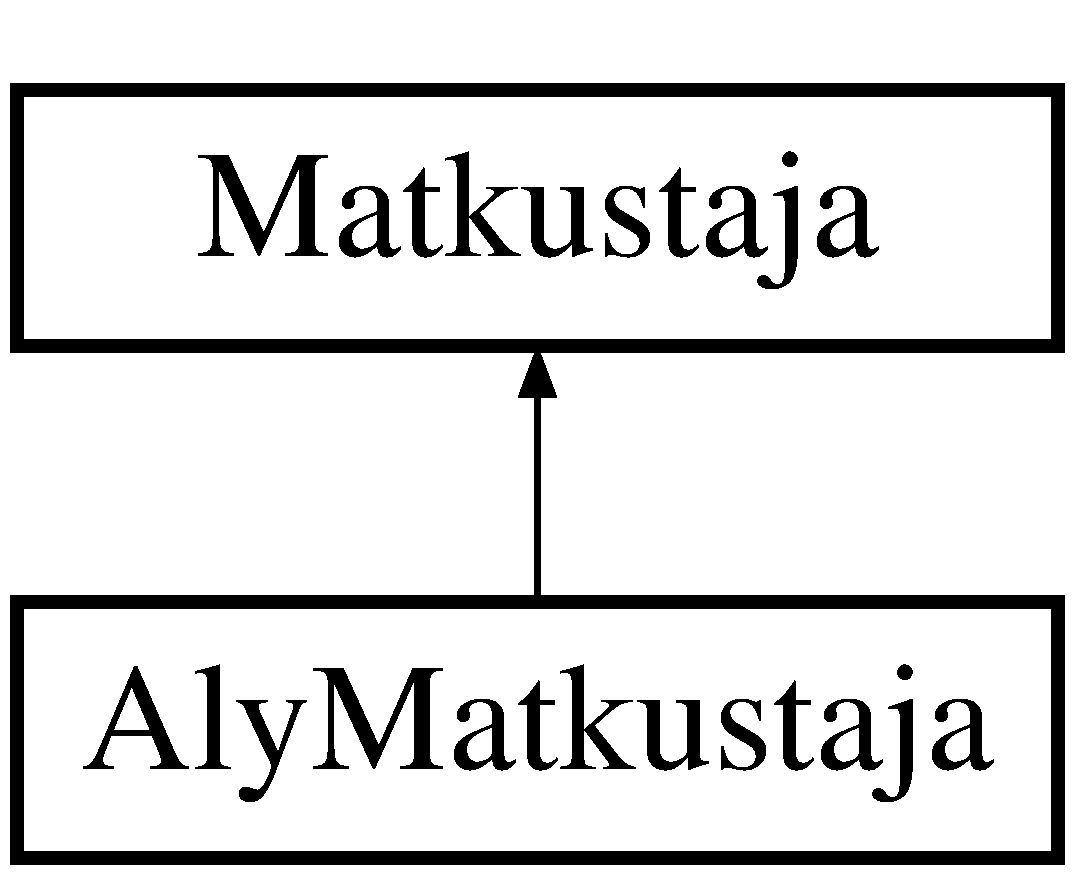
\includegraphics[height=2.000000cm]{class_aly_matkustaja}
\end{center}
\end{figure}
\subsection*{Public Member Functions}
\begin{DoxyCompactItemize}
\item 
\hypertarget{class_aly_matkustaja_a43c65df80fbb8f6a08cc64c53e937622}{virtual bool {\bfseries nousetko\-Nysseen} (std\-::weak\-\_\-ptr$<$ Nysse $>$ nysse) const }\label{class_aly_matkustaja_a43c65df80fbb8f6a08cc64c53e937622}

\item 
\hypertarget{class_aly_matkustaja_a7089b633bb040563f281310824b8ca77}{virtual bool {\bfseries menetko\-Pysakille} (std\-::weak\-\_\-ptr$<$ Rajapinta\-::\-Pysakki\-R\-P $>$) const }\label{class_aly_matkustaja_a7089b633bb040563f281310824b8ca77}

\end{DoxyCompactItemize}


The documentation for this class was generated from the following files\-:\begin{DoxyCompactItemize}
\item 
alymatkustaja.\-hh\item 
alymatkustaja.\-cpp\end{DoxyCompactItemize}

\hypertarget{class_ammus}{\section{Ammus Class Reference}
\label{class_ammus}\index{Ammus@{Ammus}}
}
Inheritance diagram for Ammus\-:\begin{figure}[H]
\begin{center}
\leavevmode
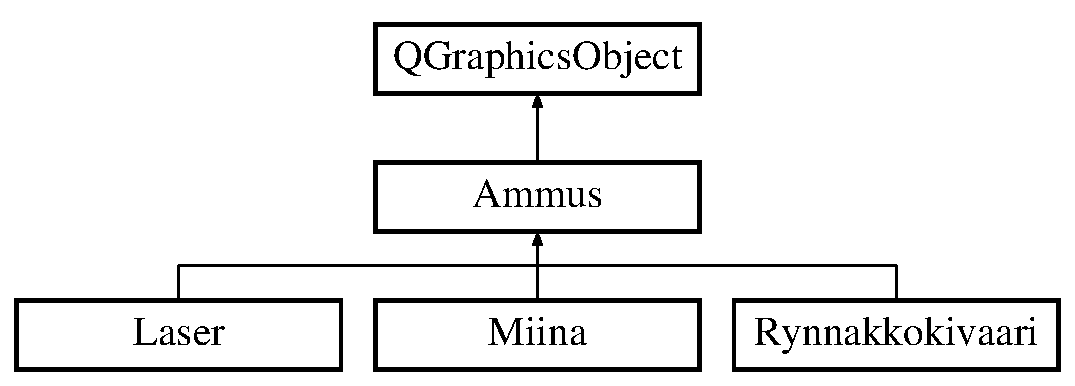
\includegraphics[height=3.000000cm]{class_ammus}
\end{center}
\end{figure}
\subsection*{Public Slots}
\begin{DoxyCompactItemize}
\item 
void \hyperlink{class_ammus_a29344837087d4864b8588e590b73732b}{tuhoa\-Ammus} ()
\begin{DoxyCompactList}\small\item\em tuhoa\-Ammus tuhoaa ammuksen hallitusti, käytetään singleshot timerin kanssa viivästettyyn tuhoamiseen. Hyödyllinen esimerkiksi animoidun räjähdyksen kanssa. \end{DoxyCompactList}\end{DoxyCompactItemize}
\subsection*{Public Member Functions}
\begin{DoxyCompactItemize}
\item 
\hypertarget{class_ammus_a7d181d103a138ac9955a612def8a68ce}{\hyperlink{class_ammus_a7d181d103a138ac9955a612def8a68ce}{Ammus} ()}\label{class_ammus_a7d181d103a138ac9955a612def8a68ce}

\begin{DoxyCompactList}\small\item\em Tyhmä rakentaja ammukselle, ei tule käyttää. \end{DoxyCompactList}\item 
\hyperlink{class_ammus_aa177444791e94b517355b6f9bce564d2}{Ammus} (Q\-Graphics\-Item $\ast$parent, qreal suunta)
\begin{DoxyCompactList}\small\item\em Ammuksen \char`\"{}perus\char`\"{} rakentaja; ei ole hyvä käyttää sinänsä, mutta toteutettu malliksi aliluokkien rakentajaksi. \end{DoxyCompactList}\item 
\hypertarget{class_ammus_a0363c773453437b858da09e72383732a}{\hyperlink{class_ammus_a0363c773453437b858da09e72383732a}{$\sim$\-Ammus} ()}\label{class_ammus_a0363c773453437b858da09e72383732a}

\begin{DoxyCompactList}\small\item\em \hyperlink{class_ammus}{Ammus} kantaluokan purkaja, hoitaa kantaluokan new'llä varaamien muuttujien tuhoamisen. \end{DoxyCompactList}\item 
virtual void \hyperlink{class_ammus_a965bb7b91b351d4ed21de577f980968d}{etene} ()
\begin{DoxyCompactList}\small\item\em etene liikuttaa ammusta ja tarkistaa mahdolliset osumat. Kantaman ylittyessä tuhoaa ammuksen. \end{DoxyCompactList}\item 
virtual void \hyperlink{class_ammus_a8863947b7cd97ddc5f0ac587547e2305}{ulko\-Osuma} ()
\begin{DoxyCompactList}\small\item\em ulko\-Osuma tuhoaa ammuksen. Käytetään kun ammus halutaan tuhota ulkopuolelta. \end{DoxyCompactList}\end{DoxyCompactItemize}
\subsection*{Protected Member Functions}
\begin{DoxyCompactItemize}
\item 
\hypertarget{class_ammus_a43f17fae41260e222e2c291ae9921516}{void {\bfseries paint} (Q\-Painter $\ast$painter, const Q\-Style\-Option\-Graphics\-Item $\ast$option, Q\-Widget $\ast$widget)}\label{class_ammus_a43f17fae41260e222e2c291ae9921516}

\item 
\hypertarget{class_ammus_ad6879b5760f9f1b00f0dad26a693bf5a}{virtual Q\-Rect\-F {\bfseries bounding\-Rect} () const }\label{class_ammus_ad6879b5760f9f1b00f0dad26a693bf5a}

\item 
virtual void \hyperlink{class_ammus_aeba3c164d8cd35b3937496904780e3f0}{alusta\-Ammus} (Q\-Graphics\-Item $\ast$parent, qreal suunta)
\begin{DoxyCompactList}\small\item\em alusta\-Ammus Alustaa ammuksen toimintakuntoon. Käynnistää ammuksen ajastimen. Kutsutaan yleensä ammuksen rakentajassa. \end{DoxyCompactList}\item 
virtual void \hyperlink{class_ammus_a637789fc7748679d5e6ceeb7bb2d24a4}{aseta\-Ammuskuva} ()=0
\begin{DoxyCompactList}\small\item\em aseta\-Ammuskuva asettaa ammuksen ulkoasun. Toteutettava periytetyssä luokassa, asetettava ammuskuva on Q\-Image Ammus\-::ammuskuva. \end{DoxyCompactList}\item 
virtual bool \hyperlink{class_ammus_a60d382b563f273bb90c60c4a5b396210}{tarkista\-Osuma} ()
\begin{DoxyCompactList}\small\item\em tarkista\-Osuma tarkistaa osuuko ammus nysseen ja osuttaessa ilmoittaa sekä ammukselle että nysselle osumasta. \end{DoxyCompactList}\item 
virtual void \hyperlink{class_ammus_a81ad352e18b9b3acebd307d5c46d40ba}{osuma} ()
\begin{DoxyCompactList}\small\item\em osuma määrittelee ammuksen (ylimääräisen) käyttäytymisen osuessa kohteeseen. Oletustoteutus ei tee mitään. \end{DoxyCompactList}\item 
Q\-Point\-F \hyperlink{class_ammus_a1195266d54d90cc1080db00ba425f717}{suunta\-Piste} () const 
\begin{DoxyCompactList}\small\item\em suunta\-Piste selvittää ammuksen etenemissuunnan. \end{DoxyCompactList}\end{DoxyCompactItemize}
\subsection*{Protected Attributes}
\begin{DoxyCompactItemize}
\item 
\hypertarget{class_ammus_a6b2e4a71e83ffc1f73d711fecd1d6e23}{Q\-Image {\bfseries ammuskuva}}\label{class_ammus_a6b2e4a71e83ffc1f73d711fecd1d6e23}

\item 
\hypertarget{class_ammus_a1f3a4778ce2af1c1204b41aef380e6fd}{bool {\bfseries animoitu\-Osuma\-\_\-} \{false\}}\label{class_ammus_a1f3a4778ce2af1c1204b41aef380e6fd}

\item 
\hypertarget{class_ammus_a6a0d35b4e038c0239400c574df51e7e2}{int {\bfseries nopeus} \{1500\}}\label{class_ammus_a6a0d35b4e038c0239400c574df51e7e2}

\item 
\hypertarget{class_ammus_a66ca908e275d08437fea7c3d30b0c6db}{int {\bfseries kantama} \{300\}}\label{class_ammus_a66ca908e275d08437fea7c3d30b0c6db}

\item 
\hypertarget{class_ammus_a5e4ee33acdc36a7c26dbcd777afb34a4}{qreal {\bfseries suunta\-\_\-} \{0\}}\label{class_ammus_a5e4ee33acdc36a7c26dbcd777afb34a4}

\item 
\hypertarget{class_ammus_aa5a5684121d62e831e4684128e75926d}{qreal {\bfseries etenema}}\label{class_ammus_aa5a5684121d62e831e4684128e75926d}

\item 
\hypertarget{class_ammus_ad34451c16b99b60a93bca9203f04165c}{Q\-Timer $\ast$ {\bfseries animaatioajastin}}\label{class_ammus_ad34451c16b99b60a93bca9203f04165c}

\item 
\hypertarget{class_ammus_af6010d25cc2e41e723470e81158c230a}{bool {\bfseries tuhoutumassa} \{false\}}\label{class_ammus_af6010d25cc2e41e723470e81158c230a}

\end{DoxyCompactItemize}


\subsection{Constructor \& Destructor Documentation}
\hypertarget{class_ammus_aa177444791e94b517355b6f9bce564d2}{\index{Ammus@{Ammus}!Ammus@{Ammus}}
\index{Ammus@{Ammus}!Ammus@{Ammus}}
\subsubsection[{Ammus}]{\setlength{\rightskip}{0pt plus 5cm}Ammus\-::\-Ammus (
\begin{DoxyParamCaption}
\item[{Q\-Graphics\-Item $\ast$}]{parent, }
\item[{qreal}]{suunta}
\end{DoxyParamCaption}
)}}\label{class_ammus_aa177444791e94b517355b6f9bce564d2}


Ammuksen \char`\"{}perus\char`\"{} rakentaja; ei ole hyvä käyttää sinänsä, mutta toteutettu malliksi aliluokkien rakentajaksi. 


\begin{DoxyParams}{Parameters}
{\em parent} & ammuksen vanhempi \\
\hline
{\em suunta} & Ammuksen lähtösuunta \\
\hline
\end{DoxyParams}
\begin{DoxyPrecond}{Precondition}
-\/ 
\end{DoxyPrecond}
\begin{DoxyPostcond}{Postcondition}
\hyperlink{class_ammus}{Ammus} on luotu, alustettu ja liikkuu 
\end{DoxyPostcond}


\subsection{Member Function Documentation}
\hypertarget{class_ammus_aeba3c164d8cd35b3937496904780e3f0}{\index{Ammus@{Ammus}!alusta\-Ammus@{alusta\-Ammus}}
\index{alusta\-Ammus@{alusta\-Ammus}!Ammus@{Ammus}}
\subsubsection[{alusta\-Ammus}]{\setlength{\rightskip}{0pt plus 5cm}void Ammus\-::alusta\-Ammus (
\begin{DoxyParamCaption}
\item[{Q\-Graphics\-Item $\ast$}]{parent, }
\item[{qreal}]{suunta}
\end{DoxyParamCaption}
)\hspace{0.3cm}{\ttfamily [protected]}, {\ttfamily [virtual]}}}\label{class_ammus_aeba3c164d8cd35b3937496904780e3f0}


alusta\-Ammus Alustaa ammuksen toimintakuntoon. Käynnistää ammuksen ajastimen. Kutsutaan yleensä ammuksen rakentajassa. 


\begin{DoxyParams}{Parameters}
{\em parent} & Ammuksen ampuja, ammuksen lähtöpaikaksi asetetaan ampujan paikka \\
\hline
{\em suunta} & Ammuksen lähtösuunta \\
\hline
\end{DoxyParams}
\begin{DoxyPrecond}{Precondition}
\hyperlink{class_ammus}{Ammus} on alustamaton 
\end{DoxyPrecond}
\begin{DoxyPostcond}{Postcondition}
\hyperlink{class_ammus}{Ammus} on alustettu ja toimintakuntoinen. Poikkeustakuu\-: perus 
\end{DoxyPostcond}


Reimplemented in \hyperlink{class_miina_aebbb38a63fadaaba6304d017cf24773c}{Miina}.

\hypertarget{class_ammus_a637789fc7748679d5e6ceeb7bb2d24a4}{\index{Ammus@{Ammus}!aseta\-Ammuskuva@{aseta\-Ammuskuva}}
\index{aseta\-Ammuskuva@{aseta\-Ammuskuva}!Ammus@{Ammus}}
\subsubsection[{aseta\-Ammuskuva}]{\setlength{\rightskip}{0pt plus 5cm}void Ammus\-::aseta\-Ammuskuva (
\begin{DoxyParamCaption}
{}
\end{DoxyParamCaption}
)\hspace{0.3cm}{\ttfamily [protected]}, {\ttfamily [pure virtual]}}}\label{class_ammus_a637789fc7748679d5e6ceeb7bb2d24a4}


aseta\-Ammuskuva asettaa ammuksen ulkoasun. Toteutettava periytetyssä luokassa, asetettava ammuskuva on Q\-Image Ammus\-::ammuskuva. 

\begin{DoxyPrecond}{Precondition}
-\/ 
\end{DoxyPrecond}
\begin{DoxyPostcond}{Postcondition}
Ammus\-::ammuskuva on asetettu. Poikkeustakuu\-: perus 
\end{DoxyPostcond}

\begin{DoxyExceptions}{Exceptions}
{\em Peli\-Virhe} & Ammuskuvan avaaminen epäonnistui. \\
\hline
\end{DoxyExceptions}


Implemented in \hyperlink{class_miina_ac7ad8b79597c7309a80e8eb25e7addc7}{Miina}, \hyperlink{class_laser_a37b0776365b937150549db54fec6ef8d}{Laser}, and \hyperlink{class_rynnakkokivaari_a3b09e5434760dd51d7aeb5834520e52d}{Rynnakkokivaari}.

\hypertarget{class_ammus_a965bb7b91b351d4ed21de577f980968d}{\index{Ammus@{Ammus}!etene@{etene}}
\index{etene@{etene}!Ammus@{Ammus}}
\subsubsection[{etene}]{\setlength{\rightskip}{0pt plus 5cm}void Ammus\-::etene (
\begin{DoxyParamCaption}
{}
\end{DoxyParamCaption}
)\hspace{0.3cm}{\ttfamily [virtual]}}}\label{class_ammus_a965bb7b91b351d4ed21de577f980968d}


etene liikuttaa ammusta ja tarkistaa mahdolliset osumat. Kantaman ylittyessä tuhoaa ammuksen. 

\begin{DoxyPrecond}{Precondition}
\hyperlink{class_ammus}{Ammus} on alustettu 
\end{DoxyPrecond}
\begin{DoxyPostcond}{Postcondition}
\hyperlink{class_ammus}{Ammus} on liikkunut ja tarkastanut osumat. Poikkeustakuu\-: perus 
\end{DoxyPostcond}
\hypertarget{class_ammus_a81ad352e18b9b3acebd307d5c46d40ba}{\index{Ammus@{Ammus}!osuma@{osuma}}
\index{osuma@{osuma}!Ammus@{Ammus}}
\subsubsection[{osuma}]{\setlength{\rightskip}{0pt plus 5cm}void Ammus\-::osuma (
\begin{DoxyParamCaption}
{}
\end{DoxyParamCaption}
)\hspace{0.3cm}{\ttfamily [protected]}, {\ttfamily [virtual]}}}\label{class_ammus_a81ad352e18b9b3acebd307d5c46d40ba}


osuma määrittelee ammuksen (ylimääräisen) käyttäytymisen osuessa kohteeseen. Oletustoteutus ei tee mitään. 

\begin{DoxyPrecond}{Precondition}
-\/ 
\end{DoxyPrecond}
\begin{DoxyPostcond}{Postcondition}
Poikkeustakuu\-: perus 
\end{DoxyPostcond}


Reimplemented in \hyperlink{class_miina_a8de75749e159593e30bb2e4367d17698}{Miina}.

\hypertarget{class_ammus_a1195266d54d90cc1080db00ba425f717}{\index{Ammus@{Ammus}!suunta\-Piste@{suunta\-Piste}}
\index{suunta\-Piste@{suunta\-Piste}!Ammus@{Ammus}}
\subsubsection[{suunta\-Piste}]{\setlength{\rightskip}{0pt plus 5cm}Q\-Point\-F Ammus\-::suunta\-Piste (
\begin{DoxyParamCaption}
{}
\end{DoxyParamCaption}
) const\hspace{0.3cm}{\ttfamily [protected]}}}\label{class_ammus_a1195266d54d90cc1080db00ba425f717}


suunta\-Piste selvittää ammuksen etenemissuunnan. 

\begin{DoxyPrecond}{Precondition}
\hyperlink{class_ammus}{Ammus} on alustettu 
\end{DoxyPrecond}
\begin{DoxyReturn}{Returns}
etäisyydellä 1 ammuksesta oleva Q\-Point\-F ammuksen etenemissuunnassa 
\end{DoxyReturn}
\begin{DoxyPostcond}{Postcondition}
Poikkeustakuu\-: perus 
\end{DoxyPostcond}
\hypertarget{class_ammus_a60d382b563f273bb90c60c4a5b396210}{\index{Ammus@{Ammus}!tarkista\-Osuma@{tarkista\-Osuma}}
\index{tarkista\-Osuma@{tarkista\-Osuma}!Ammus@{Ammus}}
\subsubsection[{tarkista\-Osuma}]{\setlength{\rightskip}{0pt plus 5cm}bool Ammus\-::tarkista\-Osuma (
\begin{DoxyParamCaption}
{}
\end{DoxyParamCaption}
)\hspace{0.3cm}{\ttfamily [protected]}, {\ttfamily [virtual]}}}\label{class_ammus_a60d382b563f273bb90c60c4a5b396210}


tarkista\-Osuma tarkistaa osuuko ammus nysseen ja osuttaessa ilmoittaa sekä ammukselle että nysselle osumasta. 

\begin{DoxyPrecond}{Precondition}
\hyperlink{class_ammus}{Ammus} on alustettu 
\end{DoxyPrecond}
\begin{DoxyReturn}{Returns}
true mikäli ammus osui, muuten false 
\end{DoxyReturn}
\begin{DoxyPostcond}{Postcondition}
Poikkeustakuu\-: perus 
\end{DoxyPostcond}


Reimplemented in \hyperlink{class_miina_a10639c013e046a6670362ac4416d3c14}{Miina}, and \hyperlink{class_laser_af022ce6822c0303e886812823e48ea82}{Laser}.

\hypertarget{class_ammus_a29344837087d4864b8588e590b73732b}{\index{Ammus@{Ammus}!tuhoa\-Ammus@{tuhoa\-Ammus}}
\index{tuhoa\-Ammus@{tuhoa\-Ammus}!Ammus@{Ammus}}
\subsubsection[{tuhoa\-Ammus}]{\setlength{\rightskip}{0pt plus 5cm}void Ammus\-::tuhoa\-Ammus (
\begin{DoxyParamCaption}
{}
\end{DoxyParamCaption}
)\hspace{0.3cm}{\ttfamily [slot]}}}\label{class_ammus_a29344837087d4864b8588e590b73732b}


tuhoa\-Ammus tuhoaa ammuksen hallitusti, käytetään singleshot timerin kanssa viivästettyyn tuhoamiseen. Hyödyllinen esimerkiksi animoidun räjähdyksen kanssa. 

\begin{DoxyPrecond}{Precondition}
\hyperlink{class_ammus}{Ammus} on alustettu 
\end{DoxyPrecond}
\begin{DoxyPostcond}{Postcondition}
\hyperlink{class_ammus}{Ammus} on tuhottu oikein. Poikkeustakuu\-: vahva 
\end{DoxyPostcond}
\hypertarget{class_ammus_a8863947b7cd97ddc5f0ac587547e2305}{\index{Ammus@{Ammus}!ulko\-Osuma@{ulko\-Osuma}}
\index{ulko\-Osuma@{ulko\-Osuma}!Ammus@{Ammus}}
\subsubsection[{ulko\-Osuma}]{\setlength{\rightskip}{0pt plus 5cm}void Ammus\-::ulko\-Osuma (
\begin{DoxyParamCaption}
{}
\end{DoxyParamCaption}
)\hspace{0.3cm}{\ttfamily [virtual]}}}\label{class_ammus_a8863947b7cd97ddc5f0ac587547e2305}


ulko\-Osuma tuhoaa ammuksen. Käytetään kun ammus halutaan tuhota ulkopuolelta. 

\begin{DoxyPrecond}{Precondition}
\hyperlink{class_ammus}{Ammus} on alustettu 
\end{DoxyPrecond}
\begin{DoxyPostcond}{Postcondition}
\hyperlink{class_ammus}{Ammus} on tuhottu normaalisti tai ajoitettu tuhoutumaan normaalisti. Poikkeustakuu\-: perus. 
\end{DoxyPostcond}


The documentation for this class was generated from the following files\-:\begin{DoxyCompactItemize}
\item 
\hyperlink{ammus_8hh}{ammus.\-hh}\item 
ammus.\-cpp\end{DoxyCompactItemize}

\hypertarget{class_drooni}{\section{Drooni Class Reference}
\label{class_drooni}\index{Drooni@{Drooni}}
}
Inheritance diagram for Drooni\-:\begin{figure}[H]
\begin{center}
\leavevmode
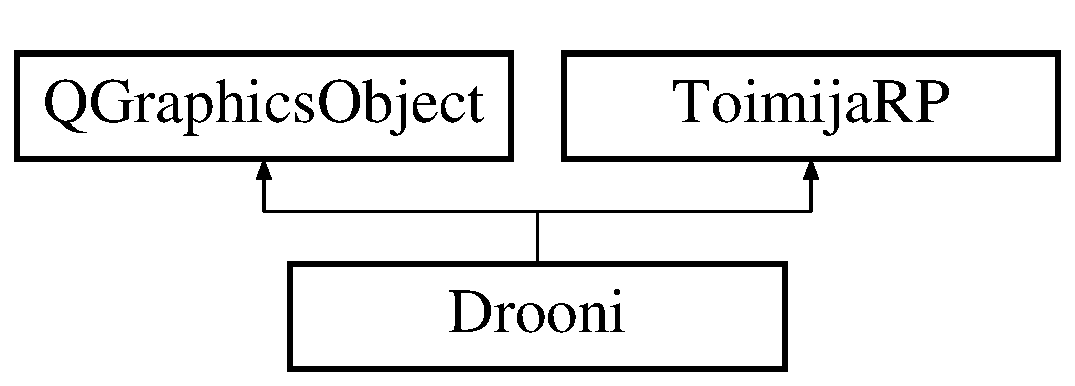
\includegraphics[height=2.000000cm]{class_drooni}
\end{center}
\end{figure}
\subsection*{Public Slots}
\begin{DoxyCompactItemize}
\item 
void \hyperlink{class_drooni_a13704789c83b2a871aa9ae0a0b8344f0}{ala\-Liikkua\-Eteen} ()
\begin{DoxyCompactList}\small\item\em ala\-Liikkua\-Eteen Laittaa droonin liikkumaan eteenpäin kunnes liike lopetetaan. \end{DoxyCompactList}\item 
void \hyperlink{class_drooni_a00017b1e9eb860c06d4422d7a60a0809}{ala\-Liikkua\-Taakse} ()
\begin{DoxyCompactList}\small\item\em ala\-Liikkua\-Taakse Laittaa droonin liikkumaan taaksepäin kunnes liike lopetetaan. \end{DoxyCompactList}\item 
void \hyperlink{class_drooni_ad1a61ea9bd674ad83267ea9259d3a807}{ala\-Kaantya\-Myota} ()
\begin{DoxyCompactList}\small\item\em ala\-Kaantya\-Myota Laittaa droonin kääntymään myötäpäivään kunnes kääntyminen lopetetaan. \end{DoxyCompactList}\item 
void \hyperlink{class_drooni_ad6bbe6b848b5e3c52afcf6b13258dc4b}{ala\-Kaantya\-Vasta} ()
\begin{DoxyCompactList}\small\item\em ala\-Kaantya\-Vasta Laittaa droonin kääntymään vastapäivään kunnes kääntyminen lopetetaan. \end{DoxyCompactList}\item 
void \hyperlink{class_drooni_ae27475e5b09619e4b635b5109f9378f9}{lopeta\-Eteen\-Liikkuminen} ()
\begin{DoxyCompactList}\small\item\em lopeta\-Eteen\-Liikkuminen Lopettaa droonin eteenpäin liikkumisen. \end{DoxyCompactList}\item 
void \hyperlink{class_drooni_ab44ae640ee3c0d47839188e0d4946d34}{lopeta\-Taakse\-Liikkuminen} ()
\begin{DoxyCompactList}\small\item\em lopeta\-Taakse\-Liikkuminen Lopettaa droonin taaksepäin liikkumisen. \end{DoxyCompactList}\item 
void \hyperlink{class_drooni_ab849dde58e4cadd190f694b0610e2215}{lopeta\-Kaannos\-Myota} ()
\begin{DoxyCompactList}\small\item\em lopeta\-Kaannos\-Myota Lopettaa droonin kääntymisen myötäpäivään. \end{DoxyCompactList}\item 
void \hyperlink{class_drooni_a269a91622768bd2c56ac1b2a94151420}{lopeta\-Kaannos\-Vasta} ()
\begin{DoxyCompactList}\small\item\em lopeta\-Kaannos\-Vasta Lopettaa droonin kääntymisen vastapäivään. \end{DoxyCompactList}\item 
void \hyperlink{class_drooni_ac4a9ca011049c1098aa462a7d773c03b}{ammu} ()
\begin{DoxyCompactList}\small\item\em ammu luo uuden valitun aseen ammuksen ja lisää sen samaan Q\-Graphics\-Scenee droonin kanssa. \end{DoxyCompactList}\item 
void \hyperlink{class_drooni_acc75f5e60f161b914dd6265e59783660}{valitse\-Rynkky} ()
\begin{DoxyCompactList}\small\item\em valitse\-Rynkky valitsee rynnäkkökiväärin aktiiviseksi aseeksi. \end{DoxyCompactList}\item 
void \hyperlink{class_drooni_a3d70e2dcad21eed191d622b573f76012}{valitse\-Miina} ()
\begin{DoxyCompactList}\small\item\em valitse\-Miina valitsee maamiinan aktiiviseksi aseeksi. \end{DoxyCompactList}\item 
void \hyperlink{class_drooni_aaf79cb0fc772cb706a190c7ce7e1c893}{valitse\-Laser} ()
\begin{DoxyCompactList}\small\item\em valitse\-Laser valitsee laserin aktiiviseksi aseeksi. \end{DoxyCompactList}\end{DoxyCompactItemize}
\subsection*{Signals}
\begin{DoxyCompactItemize}
\item 
void \hyperlink{class_drooni_a3020c56fa8b0d3bfe6c1fff40df4ab2d}{drooni\-Liikkunut} (Q\-Graphics\-Item $\ast$drooni)
\begin{DoxyCompactList}\small\item\em drooni\-Liikkunut signaali lähetetään aina kun drooni on liikkunut. \end{DoxyCompactList}\item 
void \hyperlink{class_drooni_a60161e48737707a81e74982c545b8a5d}{drooni\-Ampunut} (short int ase, short int ammuksia\-\_\-jaljella)
\begin{DoxyCompactList}\small\item\em drooni\-Ampunut signaali lähetetään aina kun drooni on ampunut. \end{DoxyCompactList}\item 
\hypertarget{class_drooni_a7ba9264caa5365a27f51035dd2892860}{void \hyperlink{class_drooni_a7ba9264caa5365a27f51035dd2892860}{ammukset\-Lopussa} ()}\label{class_drooni_a7ba9264caa5365a27f51035dd2892860}

\begin{DoxyCompactList}\small\item\em ammukset\-Lopussa signaali lähetetään kun droonin ammukset ovat lopussa. \end{DoxyCompactList}\end{DoxyCompactItemize}
\subsection*{Public Member Functions}
\begin{DoxyCompactItemize}
\item 
\hyperlink{class_drooni_a7198c6e1b9677978754f2b65804cdc6f}{Drooni} (Q\-Graphics\-Item $\ast$parent=N\-U\-L\-L)
\begin{DoxyCompactList}\small\item\em Droonin rakentaja, luo uuden drooni olion. \end{DoxyCompactList}\item 
virtual \hyperlink{class_drooni_a03b2d923119be2c5ee18fc70899aa2d8}{$\sim$\-Drooni} ()
\begin{DoxyCompactList}\small\item\em $\sim$\-Drooni tuhoaa droonin. \end{DoxyCompactList}\item 
void \hyperlink{class_drooni_ae3bbb3da2c280b4281dbcd064c4f23a5}{key\-Press\-Event} (Q\-Key\-Event $\ast$event)
\begin{DoxyCompactList}\small\item\em key\-Press\-Event vastaanottaa olion saaman näppäimistösyötteen. Muuntaa nuolinäppäimet ja välilyönnin droonin liikkeiksi. Ei yleensä tarvitse kutsua itse. \end{DoxyCompactList}\item 
void \hyperlink{class_drooni_a70338cca6bd668a3ef65938d10880ad2}{key\-Release\-Event} (Q\-Key\-Event $\ast$event)
\begin{DoxyCompactList}\small\item\em key\-Release\-Event ks. key\-Press\-Event. \end{DoxyCompactList}\item 
short int \hyperlink{class_drooni_ad825d329b1cb672145a4d01e732e5d1a}{ammuksia\-Jaljella} (int ase) const 
\begin{DoxyCompactList}\small\item\em ammuksia\-Jaljella Kertoo paljonko kysytyssä aseessa on ammuksia jäljellä \end{DoxyCompactList}\item 
\hypertarget{class_drooni_ac814aabc8942f6f3785f985143e66082}{virtual Rajapinta\-::\-Sijainti {\bfseries anna\-Sijainti} () const }\label{class_drooni_ac814aabc8942f6f3785f985143e66082}

\item 
\hypertarget{class_drooni_a1eb6face0d1454af7f6c4386f8cbe456}{virtual void {\bfseries liiku} (Rajapinta\-::\-Sijainti sij)}\label{class_drooni_a1eb6face0d1454af7f6c4386f8cbe456}

\item 
\hypertarget{class_drooni_aa054670e7c126212f5684fa7be0a1ebf}{virtual bool {\bfseries onko\-Tuhottu} () const }\label{class_drooni_aa054670e7c126212f5684fa7be0a1ebf}

\item 
\hypertarget{class_drooni_a5bfb14c85e9d186a0f207fd62d7baa1d}{virtual void {\bfseries tuhoa} ()}\label{class_drooni_a5bfb14c85e9d186a0f207fd62d7baa1d}

\item 
void \hyperlink{class_drooni_aea58ffdb85ce0db9e4778e0bdf8aea11}{liiku\-Sulavasti} (Rajapinta\-::\-Sijainti sij)
\begin{DoxyCompactList}\small\item\em liiku\-Sulavasti Laittaa droonin liikkumaan sulavasti kohti annettua sijaintia. \end{DoxyCompactList}\end{DoxyCompactItemize}
\subsection*{Public Attributes}
\begin{DoxyCompactItemize}
\item 
\hypertarget{class_drooni_a9e229d50972415a7d6cef679a6935f07}{Q\-Timer $\ast$ {\bfseries animaatioajastin}}\label{class_drooni_a9e229d50972415a7d6cef679a6935f07}

\item 
\hypertarget{class_drooni_aaf12601ff6c06afaf92e150b2e4a8741}{bool {\bfseries liikkuu\-Eteen}}\label{class_drooni_aaf12601ff6c06afaf92e150b2e4a8741}

\item 
\hypertarget{class_drooni_af963430a0c950d2a2a2635f449c80ca1}{bool {\bfseries liikkuu\-Taakse}}\label{class_drooni_af963430a0c950d2a2a2635f449c80ca1}

\item 
\hypertarget{class_drooni_a7ce57251ed439106608127008b683871}{bool {\bfseries kaantyy\-Vasemmalle}}\label{class_drooni_a7ce57251ed439106608127008b683871}

\item 
\hypertarget{class_drooni_a9419bf493ac63ff84aae5d4581e2266c}{bool {\bfseries kaantyy\-Oikealle}}\label{class_drooni_a9419bf493ac63ff84aae5d4581e2266c}

\end{DoxyCompactItemize}
\subsection*{Protected Member Functions}
\begin{DoxyCompactItemize}
\item 
\hypertarget{class_drooni_af597bf5f26942d3bdb3316386e0a187e}{void {\bfseries paint} (Q\-Painter $\ast$painter, const Q\-Style\-Option\-Graphics\-Item $\ast$option, Q\-Widget $\ast$widget)}\label{class_drooni_af597bf5f26942d3bdb3316386e0a187e}

\item 
\hypertarget{class_drooni_ae236c13bc1904e25640f1b2f8e7bfd53}{virtual Q\-Rect\-F {\bfseries bounding\-Rect} () const }\label{class_drooni_ae236c13bc1904e25640f1b2f8e7bfd53}

\item 
\hypertarget{class_drooni_a6551f75c1d307d3ef490606c7f4d2621}{virtual Q\-Variant {\bfseries item\-Change} (Graphics\-Item\-Change change, const Q\-Variant \&value)}\label{class_drooni_a6551f75c1d307d3ef490606c7f4d2621}

\end{DoxyCompactItemize}


\subsection{Constructor \& Destructor Documentation}
\hypertarget{class_drooni_a7198c6e1b9677978754f2b65804cdc6f}{\index{Drooni@{Drooni}!Drooni@{Drooni}}
\index{Drooni@{Drooni}!Drooni@{Drooni}}
\subsubsection[{Drooni}]{\setlength{\rightskip}{0pt plus 5cm}Drooni\-::\-Drooni (
\begin{DoxyParamCaption}
\item[{Q\-Graphics\-Item $\ast$}]{parent = {\ttfamily NULL}}
\end{DoxyParamCaption}
)}}\label{class_drooni_a7198c6e1b9677978754f2b65804cdc6f}


Droonin rakentaja, luo uuden drooni olion. 


\begin{DoxyParams}{Parameters}
{\em parent} & droonin vanhempi, mahdollista jättää määrittelemättä. \\
\hline
\end{DoxyParams}
\begin{DoxyPrecond}{Precondition}
-\/ 
\end{DoxyPrecond}
\begin{DoxyPostcond}{Postcondition}
\hyperlink{class_drooni}{Drooni} on luotu ja valmis käytettäväksi. Poikkeustakuu\-: ?? 
\end{DoxyPostcond}
\hypertarget{class_drooni_a03b2d923119be2c5ee18fc70899aa2d8}{\index{Drooni@{Drooni}!$\sim$\-Drooni@{$\sim$\-Drooni}}
\index{$\sim$\-Drooni@{$\sim$\-Drooni}!Drooni@{Drooni}}
\subsubsection[{$\sim$\-Drooni}]{\setlength{\rightskip}{0pt plus 5cm}Drooni\-::$\sim$\-Drooni (
\begin{DoxyParamCaption}
{}
\end{DoxyParamCaption}
)\hspace{0.3cm}{\ttfamily [virtual]}}}\label{class_drooni_a03b2d923119be2c5ee18fc70899aa2d8}


$\sim$\-Drooni tuhoaa droonin. 

\begin{DoxyPostcond}{Postcondition}
drooni on tuhottu. 
\end{DoxyPostcond}


\subsection{Member Function Documentation}
\hypertarget{class_drooni_ad1a61ea9bd674ad83267ea9259d3a807}{\index{Drooni@{Drooni}!ala\-Kaantya\-Myota@{ala\-Kaantya\-Myota}}
\index{ala\-Kaantya\-Myota@{ala\-Kaantya\-Myota}!Drooni@{Drooni}}
\subsubsection[{ala\-Kaantya\-Myota}]{\setlength{\rightskip}{0pt plus 5cm}void Drooni\-::ala\-Kaantya\-Myota (
\begin{DoxyParamCaption}
{}
\end{DoxyParamCaption}
)\hspace{0.3cm}{\ttfamily [slot]}}}\label{class_drooni_ad1a61ea9bd674ad83267ea9259d3a807}


ala\-Kaantya\-Myota Laittaa droonin kääntymään myötäpäivään kunnes kääntyminen lopetetaan. 

\begin{DoxyPrecond}{Precondition}
-\/ 
\end{DoxyPrecond}
\begin{DoxyPostcond}{Postcondition}
kaantyy\-Oikealle = true 
\end{DoxyPostcond}
\hypertarget{class_drooni_ad6bbe6b848b5e3c52afcf6b13258dc4b}{\index{Drooni@{Drooni}!ala\-Kaantya\-Vasta@{ala\-Kaantya\-Vasta}}
\index{ala\-Kaantya\-Vasta@{ala\-Kaantya\-Vasta}!Drooni@{Drooni}}
\subsubsection[{ala\-Kaantya\-Vasta}]{\setlength{\rightskip}{0pt plus 5cm}void Drooni\-::ala\-Kaantya\-Vasta (
\begin{DoxyParamCaption}
{}
\end{DoxyParamCaption}
)\hspace{0.3cm}{\ttfamily [slot]}}}\label{class_drooni_ad6bbe6b848b5e3c52afcf6b13258dc4b}


ala\-Kaantya\-Vasta Laittaa droonin kääntymään vastapäivään kunnes kääntyminen lopetetaan. 

\begin{DoxyPrecond}{Precondition}
-\/ 
\end{DoxyPrecond}
\begin{DoxyPostcond}{Postcondition}
kaantyy\-Vasemmalle = true; 
\end{DoxyPostcond}
\hypertarget{class_drooni_a13704789c83b2a871aa9ae0a0b8344f0}{\index{Drooni@{Drooni}!ala\-Liikkua\-Eteen@{ala\-Liikkua\-Eteen}}
\index{ala\-Liikkua\-Eteen@{ala\-Liikkua\-Eteen}!Drooni@{Drooni}}
\subsubsection[{ala\-Liikkua\-Eteen}]{\setlength{\rightskip}{0pt plus 5cm}void Drooni\-::ala\-Liikkua\-Eteen (
\begin{DoxyParamCaption}
{}
\end{DoxyParamCaption}
)\hspace{0.3cm}{\ttfamily [slot]}}}\label{class_drooni_a13704789c83b2a871aa9ae0a0b8344f0}


ala\-Liikkua\-Eteen Laittaa droonin liikkumaan eteenpäin kunnes liike lopetetaan. 

\begin{DoxyPrecond}{Precondition}
-\/ 
\end{DoxyPrecond}
\begin{DoxyPostcond}{Postcondition}
liikkuu\-Eteen = true 
\end{DoxyPostcond}
\hypertarget{class_drooni_a00017b1e9eb860c06d4422d7a60a0809}{\index{Drooni@{Drooni}!ala\-Liikkua\-Taakse@{ala\-Liikkua\-Taakse}}
\index{ala\-Liikkua\-Taakse@{ala\-Liikkua\-Taakse}!Drooni@{Drooni}}
\subsubsection[{ala\-Liikkua\-Taakse}]{\setlength{\rightskip}{0pt plus 5cm}void Drooni\-::ala\-Liikkua\-Taakse (
\begin{DoxyParamCaption}
{}
\end{DoxyParamCaption}
)\hspace{0.3cm}{\ttfamily [slot]}}}\label{class_drooni_a00017b1e9eb860c06d4422d7a60a0809}


ala\-Liikkua\-Taakse Laittaa droonin liikkumaan taaksepäin kunnes liike lopetetaan. 

\begin{DoxyPrecond}{Precondition}
-\/ 
\end{DoxyPrecond}
\begin{DoxyPostcond}{Postcondition}
liikkuu\-Taakse = true 
\end{DoxyPostcond}
\hypertarget{class_drooni_ac4a9ca011049c1098aa462a7d773c03b}{\index{Drooni@{Drooni}!ammu@{ammu}}
\index{ammu@{ammu}!Drooni@{Drooni}}
\subsubsection[{ammu}]{\setlength{\rightskip}{0pt plus 5cm}void Drooni\-::ammu (
\begin{DoxyParamCaption}
{}
\end{DoxyParamCaption}
)\hspace{0.3cm}{\ttfamily [slot]}}}\label{class_drooni_ac4a9ca011049c1098aa462a7d773c03b}


ammu luo uuden valitun aseen ammuksen ja lisää sen samaan Q\-Graphics\-Scenee droonin kanssa. 

\begin{DoxyPrecond}{Precondition}
\hyperlink{class_drooni}{Drooni} kuuluu Q\-Graphics\-Sceneen ja ase on valituna. 
\end{DoxyPrecond}
\begin{DoxyPostcond}{Postcondition}
Uusi ammus on luotu ja lisätty Q\-Graphics\-Sceneen. Poikkeustakuu\-: vahva 
\end{DoxyPostcond}
\hypertarget{class_drooni_ad825d329b1cb672145a4d01e732e5d1a}{\index{Drooni@{Drooni}!ammuksia\-Jaljella@{ammuksia\-Jaljella}}
\index{ammuksia\-Jaljella@{ammuksia\-Jaljella}!Drooni@{Drooni}}
\subsubsection[{ammuksia\-Jaljella}]{\setlength{\rightskip}{0pt plus 5cm}short Drooni\-::ammuksia\-Jaljella (
\begin{DoxyParamCaption}
\item[{int}]{ase}
\end{DoxyParamCaption}
) const}}\label{class_drooni_ad825d329b1cb672145a4d01e732e5d1a}


ammuksia\-Jaljella Kertoo paljonko kysytyssä aseessa on ammuksia jäljellä 


\begin{DoxyParams}{Parameters}
{\em ase} & Aseen, jonka ammustiedot halutaan, numero. 1 = R\-K, 2 = Maamiina, 3 = \hyperlink{class_laser}{Laser} \\
\hline
\end{DoxyParams}
\begin{DoxyReturn}{Returns}
Jäljellä olevien ammusten lukumäärä 
\end{DoxyReturn}
\begin{DoxyPrecond}{Precondition}
ase on välillä \mbox{[}0,2\mbox{]} 
\end{DoxyPrecond}
\begin{DoxyPostcond}{Postcondition}
Poikkeustakuu\-: vahva 
\end{DoxyPostcond}

\begin{DoxyExceptions}{Exceptions}
{\em Peli\-Virhe} & mikäli aseen tietoja ei löydy \\
\hline
\end{DoxyExceptions}
\hypertarget{class_drooni_a60161e48737707a81e74982c545b8a5d}{\index{Drooni@{Drooni}!drooni\-Ampunut@{drooni\-Ampunut}}
\index{drooni\-Ampunut@{drooni\-Ampunut}!Drooni@{Drooni}}
\subsubsection[{drooni\-Ampunut}]{\setlength{\rightskip}{0pt plus 5cm}void Drooni\-::drooni\-Ampunut (
\begin{DoxyParamCaption}
\item[{short int}]{ase, }
\item[{short int}]{ammuksia\-\_\-jaljella}
\end{DoxyParamCaption}
)\hspace{0.3cm}{\ttfamily [signal]}}}\label{class_drooni_a60161e48737707a81e74982c545b8a5d}


drooni\-Ampunut signaali lähetetään aina kun drooni on ampunut. 


\begin{DoxyParams}{Parameters}
{\em ase} & Ampumiseen käytetty ase. \\
\hline
{\em ammuksia\-\_\-jaljella} & Aseen jäljellä oleva ammusmäärä. \\
\hline
\end{DoxyParams}
\hypertarget{class_drooni_a3020c56fa8b0d3bfe6c1fff40df4ab2d}{\index{Drooni@{Drooni}!drooni\-Liikkunut@{drooni\-Liikkunut}}
\index{drooni\-Liikkunut@{drooni\-Liikkunut}!Drooni@{Drooni}}
\subsubsection[{drooni\-Liikkunut}]{\setlength{\rightskip}{0pt plus 5cm}void Drooni\-::drooni\-Liikkunut (
\begin{DoxyParamCaption}
\item[{Q\-Graphics\-Item $\ast$}]{drooni}
\end{DoxyParamCaption}
)\hspace{0.3cm}{\ttfamily [signal]}}}\label{class_drooni_a3020c56fa8b0d3bfe6c1fff40df4ab2d}


drooni\-Liikkunut signaali lähetetään aina kun drooni on liikkunut. 


\begin{DoxyParams}{Parameters}
{\em ottaa} & droonin parametrinansa. \\
\hline
\end{DoxyParams}
\hypertarget{class_drooni_ae3bbb3da2c280b4281dbcd064c4f23a5}{\index{Drooni@{Drooni}!key\-Press\-Event@{key\-Press\-Event}}
\index{key\-Press\-Event@{key\-Press\-Event}!Drooni@{Drooni}}
\subsubsection[{key\-Press\-Event}]{\setlength{\rightskip}{0pt plus 5cm}void Drooni\-::key\-Press\-Event (
\begin{DoxyParamCaption}
\item[{Q\-Key\-Event $\ast$}]{event}
\end{DoxyParamCaption}
)}}\label{class_drooni_ae3bbb3da2c280b4281dbcd064c4f23a5}


key\-Press\-Event vastaanottaa olion saaman näppäimistösyötteen. Muuntaa nuolinäppäimet ja välilyönnin droonin liikkeiksi. Ei yleensä tarvitse kutsua itse. 


\begin{DoxyParams}{Parameters}
{\em event} & Q\-Key\-Event$\ast$ tyyppinen tapahtuma. \\
\hline
\end{DoxyParams}
\begin{DoxyPrecond}{Precondition}
-\/ 
\end{DoxyPrecond}
\begin{DoxyPostcond}{Postcondition}
\hyperlink{class_drooni}{Drooni} on reagoinnut painikkeeseen halutulla tavalla. Poikkeustakuu\-: ?? 
\end{DoxyPostcond}
\hypertarget{class_drooni_a70338cca6bd668a3ef65938d10880ad2}{\index{Drooni@{Drooni}!key\-Release\-Event@{key\-Release\-Event}}
\index{key\-Release\-Event@{key\-Release\-Event}!Drooni@{Drooni}}
\subsubsection[{key\-Release\-Event}]{\setlength{\rightskip}{0pt plus 5cm}void Drooni\-::key\-Release\-Event (
\begin{DoxyParamCaption}
\item[{Q\-Key\-Event $\ast$}]{event}
\end{DoxyParamCaption}
)}}\label{class_drooni_a70338cca6bd668a3ef65938d10880ad2}


key\-Release\-Event ks. key\-Press\-Event. 


\begin{DoxyParams}{Parameters}
{\em event} & ks. key\-Press\-Event. \\
\hline
\end{DoxyParams}
\hypertarget{class_drooni_aea58ffdb85ce0db9e4778e0bdf8aea11}{\index{Drooni@{Drooni}!liiku\-Sulavasti@{liiku\-Sulavasti}}
\index{liiku\-Sulavasti@{liiku\-Sulavasti}!Drooni@{Drooni}}
\subsubsection[{liiku\-Sulavasti}]{\setlength{\rightskip}{0pt plus 5cm}void Drooni\-::liiku\-Sulavasti (
\begin{DoxyParamCaption}
\item[{Rajapinta\-::\-Sijainti}]{sij}
\end{DoxyParamCaption}
)}}\label{class_drooni_aea58ffdb85ce0db9e4778e0bdf8aea11}


liiku\-Sulavasti Laittaa droonin liikkumaan sulavasti kohti annettua sijaintia. 


\begin{DoxyParams}{Parameters}
{\em sij} & Määränpää sijainti \\
\hline
\end{DoxyParams}
\begin{DoxyPrecond}{Precondition}
-\/ 
\end{DoxyPrecond}
\begin{DoxyPostcond}{Postcondition}
\hyperlink{class_drooni}{Drooni} liikkuu kohti määränpäätä. Poikkeustakuu\-: perus 
\end{DoxyPostcond}
\hypertarget{class_drooni_ae27475e5b09619e4b635b5109f9378f9}{\index{Drooni@{Drooni}!lopeta\-Eteen\-Liikkuminen@{lopeta\-Eteen\-Liikkuminen}}
\index{lopeta\-Eteen\-Liikkuminen@{lopeta\-Eteen\-Liikkuminen}!Drooni@{Drooni}}
\subsubsection[{lopeta\-Eteen\-Liikkuminen}]{\setlength{\rightskip}{0pt plus 5cm}void Drooni\-::lopeta\-Eteen\-Liikkuminen (
\begin{DoxyParamCaption}
{}
\end{DoxyParamCaption}
)\hspace{0.3cm}{\ttfamily [slot]}}}\label{class_drooni_ae27475e5b09619e4b635b5109f9378f9}


lopeta\-Eteen\-Liikkuminen Lopettaa droonin eteenpäin liikkumisen. 

\begin{DoxyPrecond}{Precondition}
-\/ 
\end{DoxyPrecond}
\begin{DoxyPostcond}{Postcondition}
liikkuu\-Eteen = false 
\end{DoxyPostcond}
\hypertarget{class_drooni_ab849dde58e4cadd190f694b0610e2215}{\index{Drooni@{Drooni}!lopeta\-Kaannos\-Myota@{lopeta\-Kaannos\-Myota}}
\index{lopeta\-Kaannos\-Myota@{lopeta\-Kaannos\-Myota}!Drooni@{Drooni}}
\subsubsection[{lopeta\-Kaannos\-Myota}]{\setlength{\rightskip}{0pt plus 5cm}void Drooni\-::lopeta\-Kaannos\-Myota (
\begin{DoxyParamCaption}
{}
\end{DoxyParamCaption}
)\hspace{0.3cm}{\ttfamily [slot]}}}\label{class_drooni_ab849dde58e4cadd190f694b0610e2215}


lopeta\-Kaannos\-Myota Lopettaa droonin kääntymisen myötäpäivään. 

\begin{DoxyPrecond}{Precondition}
-\/ 
\end{DoxyPrecond}
\begin{DoxyPostcond}{Postcondition}
kaantyy\-Oikealle = false 
\end{DoxyPostcond}
\hypertarget{class_drooni_a269a91622768bd2c56ac1b2a94151420}{\index{Drooni@{Drooni}!lopeta\-Kaannos\-Vasta@{lopeta\-Kaannos\-Vasta}}
\index{lopeta\-Kaannos\-Vasta@{lopeta\-Kaannos\-Vasta}!Drooni@{Drooni}}
\subsubsection[{lopeta\-Kaannos\-Vasta}]{\setlength{\rightskip}{0pt plus 5cm}void Drooni\-::lopeta\-Kaannos\-Vasta (
\begin{DoxyParamCaption}
{}
\end{DoxyParamCaption}
)\hspace{0.3cm}{\ttfamily [slot]}}}\label{class_drooni_a269a91622768bd2c56ac1b2a94151420}


lopeta\-Kaannos\-Vasta Lopettaa droonin kääntymisen vastapäivään. 

\begin{DoxyPrecond}{Precondition}
-\/ 
\end{DoxyPrecond}
\begin{DoxyPostcond}{Postcondition}
kaantyy\-Vasemmalle = false 
\end{DoxyPostcond}
\hypertarget{class_drooni_ab44ae640ee3c0d47839188e0d4946d34}{\index{Drooni@{Drooni}!lopeta\-Taakse\-Liikkuminen@{lopeta\-Taakse\-Liikkuminen}}
\index{lopeta\-Taakse\-Liikkuminen@{lopeta\-Taakse\-Liikkuminen}!Drooni@{Drooni}}
\subsubsection[{lopeta\-Taakse\-Liikkuminen}]{\setlength{\rightskip}{0pt plus 5cm}void Drooni\-::lopeta\-Taakse\-Liikkuminen (
\begin{DoxyParamCaption}
{}
\end{DoxyParamCaption}
)\hspace{0.3cm}{\ttfamily [slot]}}}\label{class_drooni_ab44ae640ee3c0d47839188e0d4946d34}


lopeta\-Taakse\-Liikkuminen Lopettaa droonin taaksepäin liikkumisen. 

\begin{DoxyPrecond}{Precondition}
-\/ 
\end{DoxyPrecond}
\begin{DoxyPostcond}{Postcondition}
liikkuu\-Taakse = false 
\end{DoxyPostcond}
\hypertarget{class_drooni_aaf79cb0fc772cb706a190c7ce7e1c893}{\index{Drooni@{Drooni}!valitse\-Laser@{valitse\-Laser}}
\index{valitse\-Laser@{valitse\-Laser}!Drooni@{Drooni}}
\subsubsection[{valitse\-Laser}]{\setlength{\rightskip}{0pt plus 5cm}void Drooni\-::valitse\-Laser (
\begin{DoxyParamCaption}
{}
\end{DoxyParamCaption}
)\hspace{0.3cm}{\ttfamily [slot]}}}\label{class_drooni_aaf79cb0fc772cb706a190c7ce7e1c893}


valitse\-Laser valitsee laserin aktiiviseksi aseeksi. 

\begin{DoxyPrecond}{Precondition}
-\/ 
\end{DoxyPrecond}
\begin{DoxyPostcond}{Postcondition}
\hyperlink{class_laser}{Laser} on valittuna. Poikkeustakuu\-: vahva 
\end{DoxyPostcond}
\hypertarget{class_drooni_a3d70e2dcad21eed191d622b573f76012}{\index{Drooni@{Drooni}!valitse\-Miina@{valitse\-Miina}}
\index{valitse\-Miina@{valitse\-Miina}!Drooni@{Drooni}}
\subsubsection[{valitse\-Miina}]{\setlength{\rightskip}{0pt plus 5cm}void Drooni\-::valitse\-Miina (
\begin{DoxyParamCaption}
{}
\end{DoxyParamCaption}
)\hspace{0.3cm}{\ttfamily [slot]}}}\label{class_drooni_a3d70e2dcad21eed191d622b573f76012}


valitse\-Miina valitsee maamiinan aktiiviseksi aseeksi. 

\begin{DoxyPrecond}{Precondition}
-\/ 
\end{DoxyPrecond}
\begin{DoxyPostcond}{Postcondition}
Maamiina on valittuna. Poikkeustakuu\-: vahva 
\end{DoxyPostcond}
\hypertarget{class_drooni_acc75f5e60f161b914dd6265e59783660}{\index{Drooni@{Drooni}!valitse\-Rynkky@{valitse\-Rynkky}}
\index{valitse\-Rynkky@{valitse\-Rynkky}!Drooni@{Drooni}}
\subsubsection[{valitse\-Rynkky}]{\setlength{\rightskip}{0pt plus 5cm}void Drooni\-::valitse\-Rynkky (
\begin{DoxyParamCaption}
{}
\end{DoxyParamCaption}
)\hspace{0.3cm}{\ttfamily [slot]}}}\label{class_drooni_acc75f5e60f161b914dd6265e59783660}


valitse\-Rynkky valitsee rynnäkkökiväärin aktiiviseksi aseeksi. 

\begin{DoxyPrecond}{Precondition}
-\/ 
\end{DoxyPrecond}
\begin{DoxyPostcond}{Postcondition}
Rynnäkkökivääri on valittuna. Poikkeustakuu\-: vahva 
\end{DoxyPostcond}


The documentation for this class was generated from the following files\-:\begin{DoxyCompactItemize}
\item 
\hyperlink{drooni_8hh}{drooni.\-hh}\item 
drooni.\-cpp\end{DoxyCompactItemize}

\hypertarget{class_kaupunki}{\section{Kaupunki Class Reference}
\label{class_kaupunki}\index{Kaupunki@{Kaupunki}}
}
Inheritance diagram for Kaupunki\-:\begin{figure}[H]
\begin{center}
\leavevmode
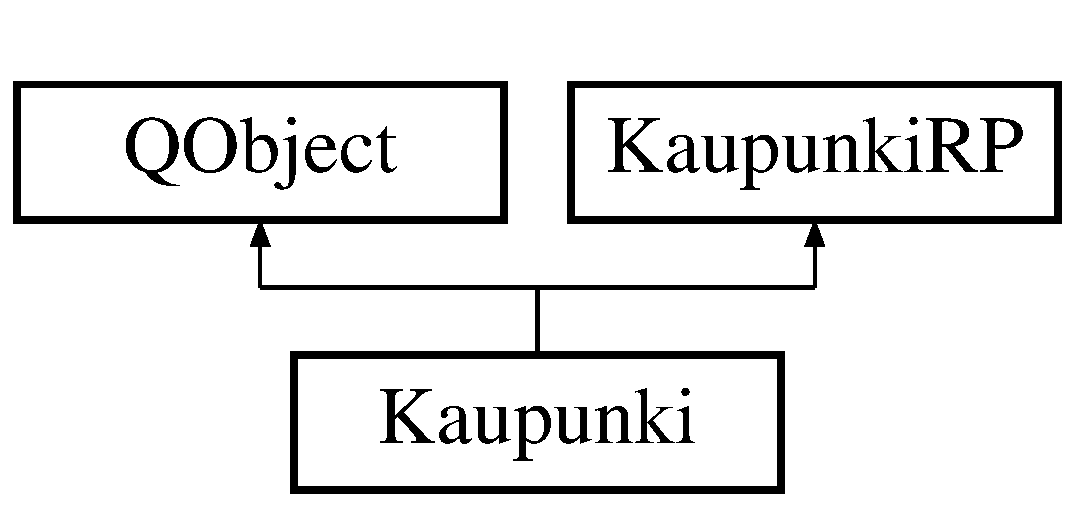
\includegraphics[height=2.000000cm]{class_kaupunki}
\end{center}
\end{figure}
\subsection*{Public Slots}
\begin{DoxyCompactItemize}
\item 
void \hyperlink{class_kaupunki_abbd4ebfe6854442610e5140023583c4d}{ajasta\-Lopetus} ()
\begin{DoxyCompactList}\small\item\em aloita\-Lopetus Käynnistää ajastimen joka X ajan kuluttua päättää pelin. Kutsutaan kun droonin ammukset loppuvat. \end{DoxyCompactList}\end{DoxyCompactItemize}
\subsection*{Public Member Functions}
\begin{DoxyCompactItemize}
\item 
\hypertarget{class_kaupunki_a2a9066295e9dcbfaba97fb677c005bc7}{virtual void {\bfseries aseta\-Tausta} (Q\-Image \&perustaustakuva, Q\-Image \&isotaustakuva)}\label{class_kaupunki_a2a9066295e9dcbfaba97fb677c005bc7}

\item 
\hypertarget{class_kaupunki_a9a93cf4868b36877ac1e427bce009231}{virtual void {\bfseries aseta\-Kello} (Q\-Time kello)}\label{class_kaupunki_a9a93cf4868b36877ac1e427bce009231}

\item 
\hypertarget{class_kaupunki_a5587a426a73729ff72e77f6024e51cdb}{virtual void {\bfseries lisaa\-Pysakki} (std\-::shared\-\_\-ptr$<$ Rajapinta\-::\-Pysakki\-R\-P $>$ pysakki)}\label{class_kaupunki_a5587a426a73729ff72e77f6024e51cdb}

\item 
\hypertarget{class_kaupunki_a3c26d0aef4079b9702df58bbe0274b8a}{virtual void {\bfseries peli\-Alkaa} ()}\label{class_kaupunki_a3c26d0aef4079b9702df58bbe0274b8a}

\item 
\hypertarget{class_kaupunki_aefd6a15df4d2bd85206cc5262b25267c}{virtual void {\bfseries lisaa\-Toimija} (std\-::shared\-\_\-ptr$<$ Rajapinta\-::\-Toimija\-R\-P $>$ uusitoimija)}\label{class_kaupunki_aefd6a15df4d2bd85206cc5262b25267c}

\item 
\hypertarget{class_kaupunki_a5860256033079dda15f83c64b5e39a27}{virtual void {\bfseries poista\-Toimija} (std\-::shared\-\_\-ptr$<$ Rajapinta\-::\-Toimija\-R\-P $>$ toimija)}\label{class_kaupunki_a5860256033079dda15f83c64b5e39a27}

\item 
\hypertarget{class_kaupunki_aeb24cf16b8f512f0a6de6599e9d70d51}{virtual void {\bfseries toimija\-Tuhottu} (std\-::shared\-\_\-ptr$<$ Rajapinta\-::\-Toimija\-R\-P $>$ toimija)}\label{class_kaupunki_aeb24cf16b8f512f0a6de6599e9d70d51}

\item 
\hypertarget{class_kaupunki_ad889a1de8dfff75075c38e41a8bf0510}{virtual bool {\bfseries loytyyko\-Toimija} (std\-::shared\-\_\-ptr$<$ Rajapinta\-::\-Toimija\-R\-P $>$ toimija) const }\label{class_kaupunki_ad889a1de8dfff75075c38e41a8bf0510}

\item 
\hypertarget{class_kaupunki_a93addb75ff5d661c627362bd93273040}{virtual void {\bfseries toimija\-Liikkunut} (std\-::shared\-\_\-ptr$<$ Rajapinta\-::\-Toimija\-R\-P $>$ toimija)}\label{class_kaupunki_a93addb75ff5d661c627362bd93273040}

\item 
\hypertarget{class_kaupunki_a3cea39227b97f25a8ea09f9540f0bba4}{virtual std\-::vector\\*
$<$ std\-::shared\-\_\-ptr\\*
$<$ Rajapinta\-::\-Toimija\-R\-P $>$ $>$ {\bfseries anna\-Toimijat\-Lahella} (Rajapinta\-::\-Sijainti paikka) const }\label{class_kaupunki_a3cea39227b97f25a8ea09f9540f0bba4}

\item 
\hypertarget{class_kaupunki_abc6aa12f2e33d21b0fb969467e9ed2ab}{virtual bool {\bfseries peli\-Loppunut} () const }\label{class_kaupunki_abc6aa12f2e33d21b0fb969467e9ed2ab}

\end{DoxyCompactItemize}


\subsection{Member Function Documentation}
\hypertarget{class_kaupunki_abbd4ebfe6854442610e5140023583c4d}{\index{Kaupunki@{Kaupunki}!ajasta\-Lopetus@{ajasta\-Lopetus}}
\index{ajasta\-Lopetus@{ajasta\-Lopetus}!Kaupunki@{Kaupunki}}
\subsubsection[{ajasta\-Lopetus}]{\setlength{\rightskip}{0pt plus 5cm}void Kaupunki\-::ajasta\-Lopetus (
\begin{DoxyParamCaption}
{}
\end{DoxyParamCaption}
)\hspace{0.3cm}{\ttfamily [slot]}}}\label{class_kaupunki_abbd4ebfe6854442610e5140023583c4d}


aloita\-Lopetus Käynnistää ajastimen joka X ajan kuluttua päättää pelin. Kutsutaan kun droonin ammukset loppuvat. 

\begin{DoxyPrecond}{Precondition}
Peli on käynnissä 
\end{DoxyPrecond}
\begin{DoxyPostcond}{Postcondition}
Peli on ajastettu loppumaan 
\end{DoxyPostcond}


The documentation for this class was generated from the following files\-:\begin{DoxyCompactItemize}
\item 
\hyperlink{kaupunki_8hh}{kaupunki.\-hh}\item 
kaupunki.\-cpp\end{DoxyCompactItemize}

\hypertarget{class_laser}{\section{Laser Class Reference}
\label{class_laser}\index{Laser@{Laser}}
}
Inheritance diagram for Laser\-:\begin{figure}[H]
\begin{center}
\leavevmode
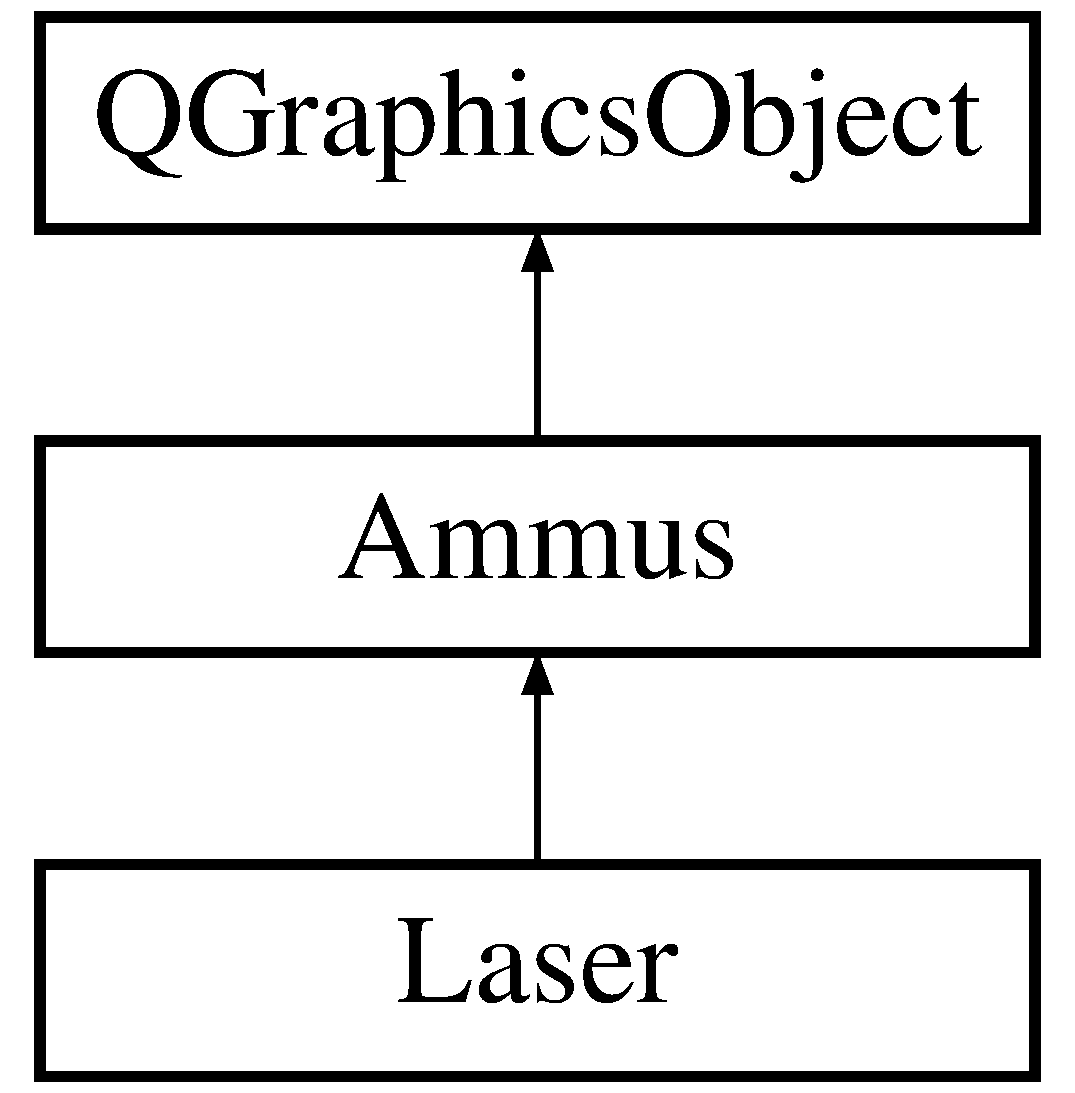
\includegraphics[height=3.000000cm]{class_laser}
\end{center}
\end{figure}
\subsection*{Public Member Functions}
\begin{DoxyCompactItemize}
\item 
\hyperlink{class_laser_a1e883d8dab1efcaf1ef692056664b080}{Laser} (Q\-Graphics\-Item $\ast$parent, qreal suunta)
\begin{DoxyCompactList}\small\item\em Laserin rakentaja. \end{DoxyCompactList}\item 
\hyperlink{class_laser_aa9baee5ed9775426e0b1d563c4687711}{$\sim$\-Laser} ()
\begin{DoxyCompactList}\small\item\em Laserin purkaja. \end{DoxyCompactList}\end{DoxyCompactItemize}
\subsection*{Protected Member Functions}
\begin{DoxyCompactItemize}
\item 
\hypertarget{class_laser_aba0ac53926bf1622172713549e6ded45}{void {\bfseries paint} (Q\-Painter $\ast$painter, const Q\-Style\-Option\-Graphics\-Item $\ast$option, Q\-Widget $\ast$widget)}\label{class_laser_aba0ac53926bf1622172713549e6ded45}

\item 
\hypertarget{class_laser_aae435ce15a186fa1dc23892ceaa2fa20}{virtual Q\-Rect\-F {\bfseries bounding\-Rect} () const override}\label{class_laser_aae435ce15a186fa1dc23892ceaa2fa20}

\item 
virtual void \hyperlink{class_laser_a37b0776365b937150549db54fec6ef8d}{aseta\-Ammuskuva} ()
\begin{DoxyCompactList}\small\item\em aseta\-Ammuskuva asettaa ammuksen ulkoasun. Toteutettava periytetyssä luokassa, asetettava ammuskuva on Q\-Image Ammus\-::ammuskuva. \end{DoxyCompactList}\item 
virtual bool \hyperlink{class_laser_af022ce6822c0303e886812823e48ea82}{tarkista\-Osuma} ()
\begin{DoxyCompactList}\small\item\em tarkista\-Osuma tarkistaa osuuko ammus nysseen ja osuttaessa ilmoittaa sekä ammukselle että nysselle osumasta. \end{DoxyCompactList}\end{DoxyCompactItemize}
\subsection*{Additional Inherited Members}


\subsection{Constructor \& Destructor Documentation}
\hypertarget{class_laser_a1e883d8dab1efcaf1ef692056664b080}{\index{Laser@{Laser}!Laser@{Laser}}
\index{Laser@{Laser}!Laser@{Laser}}
\subsubsection[{Laser}]{\setlength{\rightskip}{0pt plus 5cm}Laser\-::\-Laser (
\begin{DoxyParamCaption}
\item[{Q\-Graphics\-Item $\ast$}]{parent, }
\item[{qreal}]{suunta}
\end{DoxyParamCaption}
)}}\label{class_laser_a1e883d8dab1efcaf1ef692056664b080}


Laserin rakentaja. 


\begin{DoxyParams}{Parameters}
{\em parent} & laserin ampunut toimija, yleensä drooni \\
\hline
{\em suunta} & suunta minne laser lähtee \\
\hline
\end{DoxyParams}
\begin{DoxyPostcond}{Postcondition}
\hyperlink{class_laser}{Laser} luotu onnistuneesti ja ajoitettu tuhoutumaan 200ms kuluttua. Poikkeustakuu\-: perus 
\end{DoxyPostcond}
\hypertarget{class_laser_aa9baee5ed9775426e0b1d563c4687711}{\index{Laser@{Laser}!$\sim$\-Laser@{$\sim$\-Laser}}
\index{$\sim$\-Laser@{$\sim$\-Laser}!Laser@{Laser}}
\subsubsection[{$\sim$\-Laser}]{\setlength{\rightskip}{0pt plus 5cm}Laser\-::$\sim$\-Laser (
\begin{DoxyParamCaption}
{}
\end{DoxyParamCaption}
)}}\label{class_laser_aa9baee5ed9775426e0b1d563c4687711}


Laserin purkaja. 

\begin{DoxyPostcond}{Postcondition}
\hyperlink{class_laser}{Laser} on tuhottu oikein 
\end{DoxyPostcond}


\subsection{Member Function Documentation}
\hypertarget{class_laser_a37b0776365b937150549db54fec6ef8d}{\index{Laser@{Laser}!aseta\-Ammuskuva@{aseta\-Ammuskuva}}
\index{aseta\-Ammuskuva@{aseta\-Ammuskuva}!Laser@{Laser}}
\subsubsection[{aseta\-Ammuskuva}]{\setlength{\rightskip}{0pt plus 5cm}void Laser\-::aseta\-Ammuskuva (
\begin{DoxyParamCaption}
{}
\end{DoxyParamCaption}
)\hspace{0.3cm}{\ttfamily [protected]}, {\ttfamily [virtual]}}}\label{class_laser_a37b0776365b937150549db54fec6ef8d}


aseta\-Ammuskuva asettaa ammuksen ulkoasun. Toteutettava periytetyssä luokassa, asetettava ammuskuva on Q\-Image Ammus\-::ammuskuva. 

\begin{DoxyPrecond}{Precondition}
-\/ 
\end{DoxyPrecond}
\begin{DoxyPostcond}{Postcondition}
Ammus\-::ammuskuva on asetettu. Poikkeustakuu\-: perus 
\end{DoxyPostcond}

\begin{DoxyExceptions}{Exceptions}
{\em Peli\-Virhe} & Ammuskuvan avaaminen epäonnistui. \\
\hline
\end{DoxyExceptions}


Implements \hyperlink{class_ammus_a637789fc7748679d5e6ceeb7bb2d24a4}{Ammus}.

\hypertarget{class_laser_af022ce6822c0303e886812823e48ea82}{\index{Laser@{Laser}!tarkista\-Osuma@{tarkista\-Osuma}}
\index{tarkista\-Osuma@{tarkista\-Osuma}!Laser@{Laser}}
\subsubsection[{tarkista\-Osuma}]{\setlength{\rightskip}{0pt plus 5cm}bool Laser\-::tarkista\-Osuma (
\begin{DoxyParamCaption}
{}
\end{DoxyParamCaption}
)\hspace{0.3cm}{\ttfamily [protected]}, {\ttfamily [virtual]}}}\label{class_laser_af022ce6822c0303e886812823e48ea82}


tarkista\-Osuma tarkistaa osuuko ammus nysseen ja osuttaessa ilmoittaa sekä ammukselle että nysselle osumasta. 

\begin{DoxyPrecond}{Precondition}
\hyperlink{class_ammus}{Ammus} on alustettu 
\end{DoxyPrecond}
\begin{DoxyReturn}{Returns}
true mikäli ammus osui, muuten false 
\end{DoxyReturn}
\begin{DoxyPostcond}{Postcondition}
Poikkeustakuu\-: perus 
\end{DoxyPostcond}


Reimplemented from \hyperlink{class_ammus_a60d382b563f273bb90c60c4a5b396210}{Ammus}.



The documentation for this class was generated from the following files\-:\begin{DoxyCompactItemize}
\item 
\hyperlink{laser_8hh}{laser.\-hh}\item 
laser.\-cpp\end{DoxyCompactItemize}

\hypertarget{class_lopetus_dialog}{\section{Lopetus\-Dialog Class Reference}
\label{class_lopetus_dialog}\index{Lopetus\-Dialog@{Lopetus\-Dialog}}
}
Inheritance diagram for Lopetus\-Dialog\-:\begin{figure}[H]
\begin{center}
\leavevmode
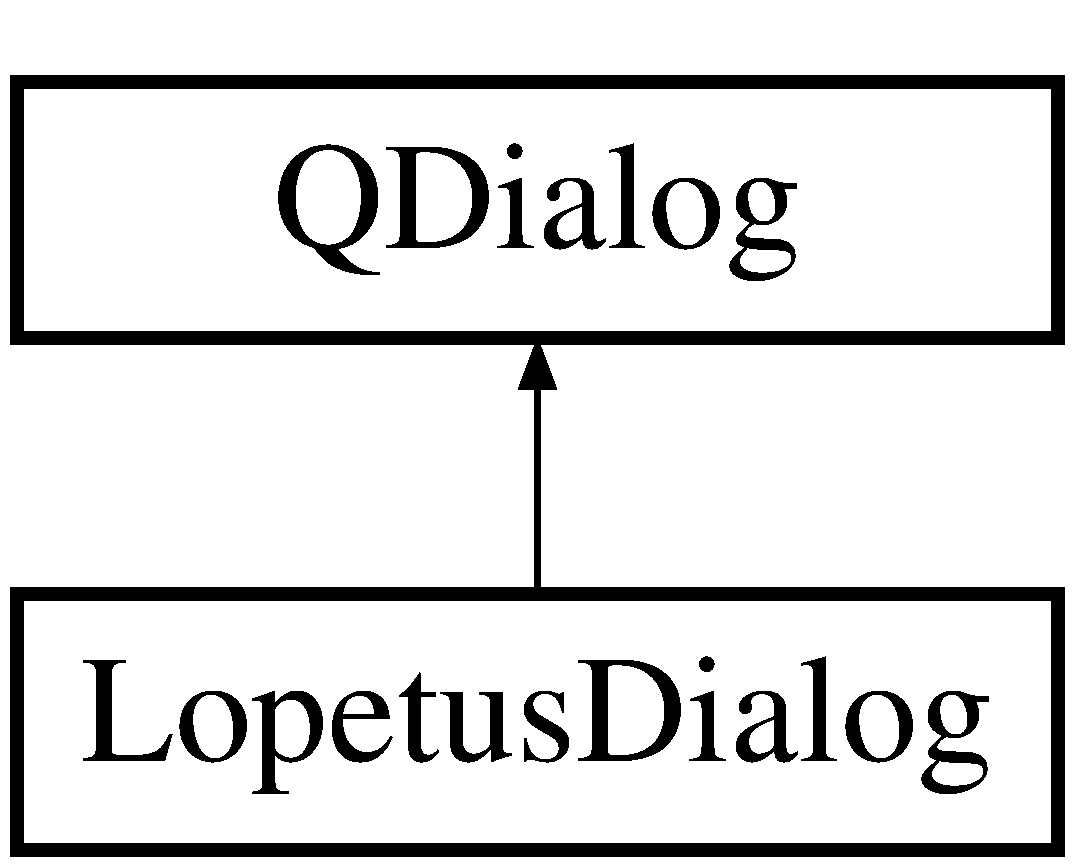
\includegraphics[height=2.000000cm]{class_lopetus_dialog}
\end{center}
\end{figure}
\subsection*{Public Member Functions}
\begin{DoxyCompactItemize}
\item 
\hypertarget{class_lopetus_dialog_a2ca8a56e125b6c129ed8b941df22f851}{{\bfseries Lopetus\-Dialog} (Q\-Widget $\ast$parent=0)}\label{class_lopetus_dialog_a2ca8a56e125b6c129ed8b941df22f851}

\item 
\hypertarget{class_lopetus_dialog_a5aa4bd894a906205a11981a5a27c7100}{void {\bfseries anna\-Tilasto} (std\-::shared\-\_\-ptr$<$ \hyperlink{class_tilasto}{Tilasto} $>$ tilastoptr)}\label{class_lopetus_dialog_a5aa4bd894a906205a11981a5a27c7100}

\item 
\hypertarget{class_lopetus_dialog_a31810cde5beafe0052d88b4eecc2d4d6}{void {\bfseries tallenna\-Ja\-Lopeta} ()}\label{class_lopetus_dialog_a31810cde5beafe0052d88b4eecc2d4d6}

\end{DoxyCompactItemize}


The documentation for this class was generated from the following files\-:\begin{DoxyCompactItemize}
\item 
lopetusdialog.\-hh\item 
lopetusdialog.\-cpp\end{DoxyCompactItemize}

\hypertarget{class_miina}{\section{Miina Class Reference}
\label{class_miina}\index{Miina@{Miina}}
}
Inheritance diagram for Miina\-:\begin{figure}[H]
\begin{center}
\leavevmode
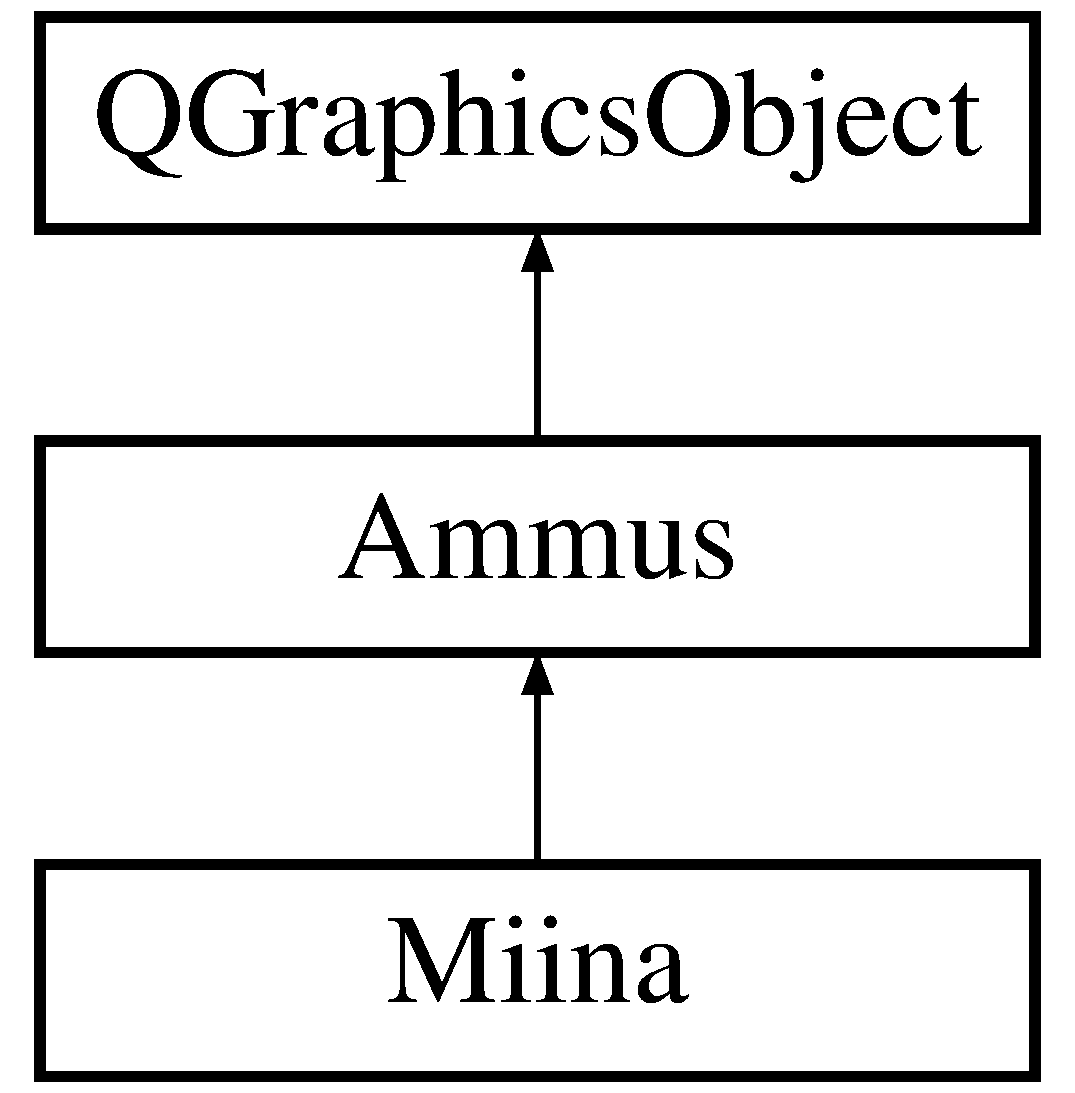
\includegraphics[height=3.000000cm]{class_miina}
\end{center}
\end{figure}
\subsection*{Public Member Functions}
\begin{DoxyCompactItemize}
\item 
\hyperlink{class_miina_aa6504bc6417688ddd65e3240118b69c9}{Miina} (Q\-Graphics\-Item $\ast$parent)
\begin{DoxyCompactList}\small\item\em Miinan rakentaja. \end{DoxyCompactList}\item 
\hyperlink{class_miina_adb79c83dd78271191b40bf7700d663db}{$\sim$\-Miina} ()
\begin{DoxyCompactList}\small\item\em Miinan purkaja. \end{DoxyCompactList}\item 
\hypertarget{class_miina_ad05abb5a4a0da5b960bc418158fc7c75}{int {\bfseries get\-Rajahdys\-Vaihe} () const }\label{class_miina_ad05abb5a4a0da5b960bc418158fc7c75}

\item 
\hypertarget{class_miina_aae598593480355a3ad261423564f035e}{void {\bfseries set\-Rajahdys\-Vaihe} (int rajahdys\-Vaihe)}\label{class_miina_aae598593480355a3ad261423564f035e}

\end{DoxyCompactItemize}
\subsection*{Protected Member Functions}
\begin{DoxyCompactItemize}
\item 
virtual void \hyperlink{class_miina_ac7ad8b79597c7309a80e8eb25e7addc7}{aseta\-Ammuskuva} ()
\begin{DoxyCompactList}\small\item\em aseta\-Ammuskuva asettaa ammuksen ulkoasun. Toteutettava periytetyssä luokassa, asetettava ammuskuva on Q\-Image Ammus\-::ammuskuva. \end{DoxyCompactList}\item 
virtual void \hyperlink{class_miina_aebbb38a63fadaaba6304d017cf24773c}{alusta\-Ammus} (Q\-Graphics\-Item $\ast$parent, qreal suunta)
\begin{DoxyCompactList}\small\item\em alusta\-Ammus Alustaa ammuksen toimintakuntoon. Käynnistää ammuksen ajastimen. Kutsutaan yleensä ammuksen rakentajassa. \end{DoxyCompactList}\item 
virtual void \hyperlink{class_miina_a8de75749e159593e30bb2e4367d17698}{osuma} ()
\begin{DoxyCompactList}\small\item\em osuma määrittelee ammuksen (ylimääräisen) käyttäytymisen osuessa kohteeseen. Oletustoteutus ei tee mitään. \end{DoxyCompactList}\item 
virtual bool \hyperlink{class_miina_a10639c013e046a6670362ac4416d3c14}{tarkista\-Osuma} ()
\begin{DoxyCompactList}\small\item\em tarkista\-Osuma tarkistaa osuuko ammus nysseen ja osuttaessa ilmoittaa sekä ammukselle että nysselle osumasta. \end{DoxyCompactList}\end{DoxyCompactItemize}
\subsection*{Properties}
\begin{DoxyCompactItemize}
\item 
\hypertarget{class_miina_a10138792eda0d168cb35b8737eddec96}{int {\bfseries r\-Vaihe}}\label{class_miina_a10138792eda0d168cb35b8737eddec96}

\end{DoxyCompactItemize}
\subsection*{Additional Inherited Members}


\subsection{Constructor \& Destructor Documentation}
\hypertarget{class_miina_aa6504bc6417688ddd65e3240118b69c9}{\index{Miina@{Miina}!Miina@{Miina}}
\index{Miina@{Miina}!Miina@{Miina}}
\subsubsection[{Miina}]{\setlength{\rightskip}{0pt plus 5cm}Miina\-::\-Miina (
\begin{DoxyParamCaption}
\item[{Q\-Graphics\-Item $\ast$}]{parent}
\end{DoxyParamCaption}
)}}\label{class_miina_aa6504bc6417688ddd65e3240118b69c9}


Miinan rakentaja. 


\begin{DoxyParams}{Parameters}
{\em parent} & miinan jättäjä, yleensä drooni \\
\hline
\end{DoxyParams}
\begin{DoxyPostcond}{Postcondition}
\hyperlink{class_miina}{Miina} asetettu ja alustettu. Poikkeustakuu\-: perus 
\end{DoxyPostcond}
\hypertarget{class_miina_adb79c83dd78271191b40bf7700d663db}{\index{Miina@{Miina}!$\sim$\-Miina@{$\sim$\-Miina}}
\index{$\sim$\-Miina@{$\sim$\-Miina}!Miina@{Miina}}
\subsubsection[{$\sim$\-Miina}]{\setlength{\rightskip}{0pt plus 5cm}Miina\-::$\sim$\-Miina (
\begin{DoxyParamCaption}
{}
\end{DoxyParamCaption}
)}}\label{class_miina_adb79c83dd78271191b40bf7700d663db}


Miinan purkaja. 

\begin{DoxyPostcond}{Postcondition}
miina on tuhottu oikein 
\end{DoxyPostcond}


\subsection{Member Function Documentation}
\hypertarget{class_miina_aebbb38a63fadaaba6304d017cf24773c}{\index{Miina@{Miina}!alusta\-Ammus@{alusta\-Ammus}}
\index{alusta\-Ammus@{alusta\-Ammus}!Miina@{Miina}}
\subsubsection[{alusta\-Ammus}]{\setlength{\rightskip}{0pt plus 5cm}void Miina\-::alusta\-Ammus (
\begin{DoxyParamCaption}
\item[{Q\-Graphics\-Item $\ast$}]{parent, }
\item[{qreal}]{suunta}
\end{DoxyParamCaption}
)\hspace{0.3cm}{\ttfamily [protected]}, {\ttfamily [virtual]}}}\label{class_miina_aebbb38a63fadaaba6304d017cf24773c}


alusta\-Ammus Alustaa ammuksen toimintakuntoon. Käynnistää ammuksen ajastimen. Kutsutaan yleensä ammuksen rakentajassa. 


\begin{DoxyParams}{Parameters}
{\em parent} & Ammuksen ampuja, ammuksen lähtöpaikaksi asetetaan ampujan paikka \\
\hline
{\em suunta} & Ammuksen lähtösuunta \\
\hline
\end{DoxyParams}
\begin{DoxyPrecond}{Precondition}
\hyperlink{class_ammus}{Ammus} on alustamaton 
\end{DoxyPrecond}
\begin{DoxyPostcond}{Postcondition}
\hyperlink{class_ammus}{Ammus} on alustettu ja toimintakuntoinen. Poikkeustakuu\-: perus 
\end{DoxyPostcond}


Reimplemented from \hyperlink{class_ammus_aeba3c164d8cd35b3937496904780e3f0}{Ammus}.

\hypertarget{class_miina_ac7ad8b79597c7309a80e8eb25e7addc7}{\index{Miina@{Miina}!aseta\-Ammuskuva@{aseta\-Ammuskuva}}
\index{aseta\-Ammuskuva@{aseta\-Ammuskuva}!Miina@{Miina}}
\subsubsection[{aseta\-Ammuskuva}]{\setlength{\rightskip}{0pt plus 5cm}void Miina\-::aseta\-Ammuskuva (
\begin{DoxyParamCaption}
{}
\end{DoxyParamCaption}
)\hspace{0.3cm}{\ttfamily [protected]}, {\ttfamily [virtual]}}}\label{class_miina_ac7ad8b79597c7309a80e8eb25e7addc7}


aseta\-Ammuskuva asettaa ammuksen ulkoasun. Toteutettava periytetyssä luokassa, asetettava ammuskuva on Q\-Image Ammus\-::ammuskuva. 

\begin{DoxyPrecond}{Precondition}
-\/ 
\end{DoxyPrecond}
\begin{DoxyPostcond}{Postcondition}
Ammus\-::ammuskuva on asetettu. Poikkeustakuu\-: perus 
\end{DoxyPostcond}

\begin{DoxyExceptions}{Exceptions}
{\em Peli\-Virhe} & Ammuskuvan avaaminen epäonnistui. \\
\hline
\end{DoxyExceptions}


Implements \hyperlink{class_ammus_a637789fc7748679d5e6ceeb7bb2d24a4}{Ammus}.

\hypertarget{class_miina_a8de75749e159593e30bb2e4367d17698}{\index{Miina@{Miina}!osuma@{osuma}}
\index{osuma@{osuma}!Miina@{Miina}}
\subsubsection[{osuma}]{\setlength{\rightskip}{0pt plus 5cm}void Miina\-::osuma (
\begin{DoxyParamCaption}
{}
\end{DoxyParamCaption}
)\hspace{0.3cm}{\ttfamily [protected]}, {\ttfamily [virtual]}}}\label{class_miina_a8de75749e159593e30bb2e4367d17698}


osuma määrittelee ammuksen (ylimääräisen) käyttäytymisen osuessa kohteeseen. Oletustoteutus ei tee mitään. 

\begin{DoxyPrecond}{Precondition}
-\/ 
\end{DoxyPrecond}
\begin{DoxyPostcond}{Postcondition}
Poikkeustakuu\-: perus 
\end{DoxyPostcond}


Reimplemented from \hyperlink{class_ammus_a81ad352e18b9b3acebd307d5c46d40ba}{Ammus}.

\hypertarget{class_miina_a10639c013e046a6670362ac4416d3c14}{\index{Miina@{Miina}!tarkista\-Osuma@{tarkista\-Osuma}}
\index{tarkista\-Osuma@{tarkista\-Osuma}!Miina@{Miina}}
\subsubsection[{tarkista\-Osuma}]{\setlength{\rightskip}{0pt plus 5cm}bool Miina\-::tarkista\-Osuma (
\begin{DoxyParamCaption}
{}
\end{DoxyParamCaption}
)\hspace{0.3cm}{\ttfamily [protected]}, {\ttfamily [virtual]}}}\label{class_miina_a10639c013e046a6670362ac4416d3c14}


tarkista\-Osuma tarkistaa osuuko ammus nysseen ja osuttaessa ilmoittaa sekä ammukselle että nysselle osumasta. 

\begin{DoxyPrecond}{Precondition}
\hyperlink{class_ammus}{Ammus} on alustettu 
\end{DoxyPrecond}
\begin{DoxyReturn}{Returns}
true mikäli ammus osui, muuten false 
\end{DoxyReturn}
\begin{DoxyPostcond}{Postcondition}
Poikkeustakuu\-: perus 
\end{DoxyPostcond}


Reimplemented from \hyperlink{class_ammus_a60d382b563f273bb90c60c4a5b396210}{Ammus}.



The documentation for this class was generated from the following files\-:\begin{DoxyCompactItemize}
\item 
\hyperlink{miina_8hh}{miina.\-hh}\item 
miina.\-cpp\end{DoxyCompactItemize}

\hypertarget{class_nyssekuva}{\section{Nyssekuva Class Reference}
\label{class_nyssekuva}\index{Nyssekuva@{Nyssekuva}}
}
Inheritance diagram for Nyssekuva\-:\begin{figure}[H]
\begin{center}
\leavevmode
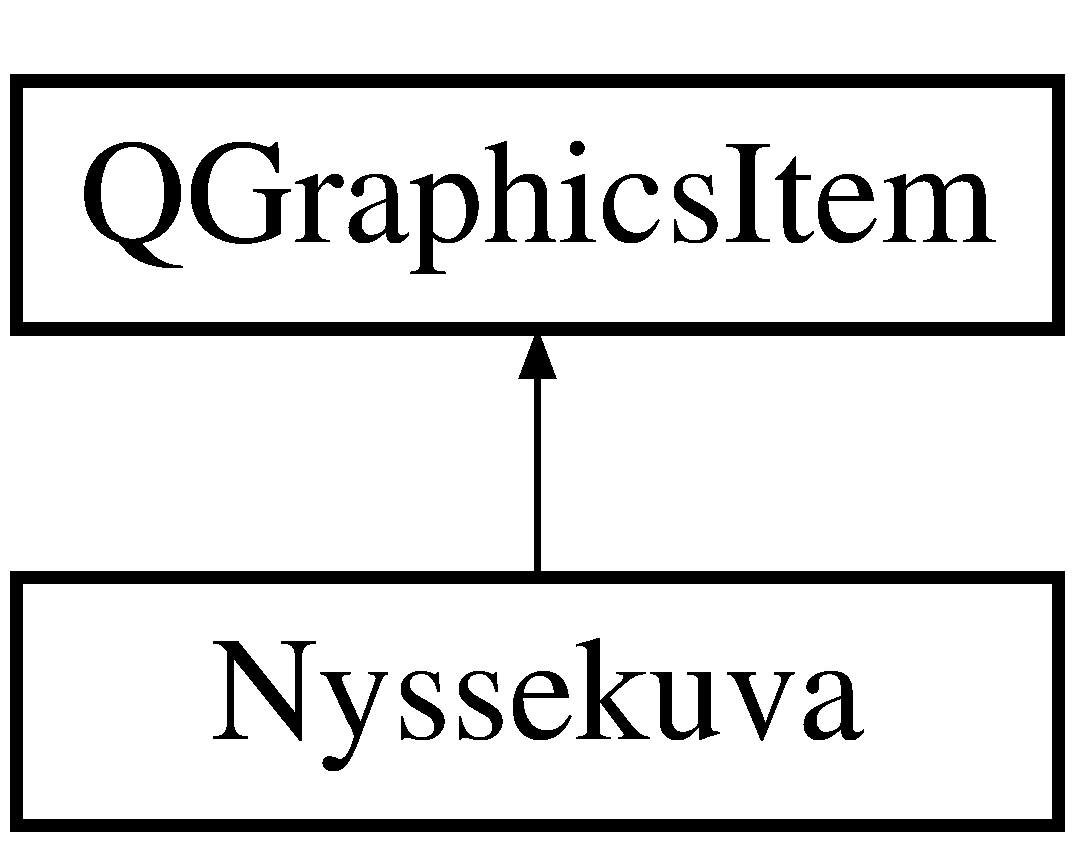
\includegraphics[height=2.000000cm]{class_nyssekuva}
\end{center}
\end{figure}
\subsection*{Public Member Functions}
\begin{DoxyCompactItemize}
\item 
\hyperlink{class_nyssekuva_a15c81255af4f21daabdc79eb7369c274}{Nyssekuva} (std\-::shared\-\_\-ptr$<$ Rajapinta\-::\-Toimija\-R\-P $>$ nysse)
\begin{DoxyCompactList}\small\item\em \hyperlink{class_nyssekuva}{Nyssekuva} Luokan rakentaja. \end{DoxyCompactList}\item 
\hyperlink{class_nyssekuva_a042ecc1e24eec8b66458c638fd6b68b1}{$\sim$\-Nyssekuva} ()
\begin{DoxyCompactList}\small\item\em Luokan purkaja. \end{DoxyCompactList}\item 
void \hyperlink{class_nyssekuva_aab047a42f0f69bf37daded779a1a1dee}{osuma} ()
\begin{DoxyCompactList}\small\item\em osuma Kutsutaan kun nysse on ottanut osuman ammuksesta. Ilmoittaa pelilogiikan nysselle tuhoutumisesta (Tuhoaa toimijan ja kertoo kaupungille) \end{DoxyCompactList}\item 
void \hyperlink{class_nyssekuva_a02b8f283b6ccacd0afe435d9eccd728b}{kerro\-Kaupunki} (Rajapinta\-::\-Kaupunki\-R\-P $\ast$kaupunki)
\begin{DoxyCompactList}\small\item\em kerro\-Kaupunki kertoo Nyssekuvalle missä kaupungissa se on. \end{DoxyCompactList}\item 
void \hyperlink{class_nyssekuva_a4d88edacd7a24757ad89253fe95caa5e}{tuhoudu} ()
\begin{DoxyCompactList}\small\item\em tuhoudu Vaihtaa nyssekuvan ulkoasun tuhoutuneeseen nysseen. \end{DoxyCompactList}\item 
bool \hyperlink{class_nyssekuva_acfa9ae5331b43f8bfec01d8c0c57c221}{tuhottu} ()
\begin{DoxyCompactList}\small\item\em tuhottu Kertoo onko Nyssekuvan ulkoasu tuhoutunut nysse. \end{DoxyCompactList}\end{DoxyCompactItemize}
\subsection*{Protected Member Functions}
\begin{DoxyCompactItemize}
\item 
\hypertarget{class_nyssekuva_a597cf4646389f6bca4fabdd96fc24b53}{void {\bfseries paint} (Q\-Painter $\ast$painter, const Q\-Style\-Option\-Graphics\-Item $\ast$option, Q\-Widget $\ast$widget)}\label{class_nyssekuva_a597cf4646389f6bca4fabdd96fc24b53}

\item 
\hypertarget{class_nyssekuva_a00b6cd60afdf8244320e5995fa639674}{virtual Q\-Rect\-F {\bfseries bounding\-Rect} () const }\label{class_nyssekuva_a00b6cd60afdf8244320e5995fa639674}

\end{DoxyCompactItemize}


\subsection{Constructor \& Destructor Documentation}
\hypertarget{class_nyssekuva_a15c81255af4f21daabdc79eb7369c274}{\index{Nyssekuva@{Nyssekuva}!Nyssekuva@{Nyssekuva}}
\index{Nyssekuva@{Nyssekuva}!Nyssekuva@{Nyssekuva}}
\subsubsection[{Nyssekuva}]{\setlength{\rightskip}{0pt plus 5cm}Nyssekuva\-::\-Nyssekuva (
\begin{DoxyParamCaption}
\item[{std\-::shared\-\_\-ptr$<$ Rajapinta\-::\-Toimija\-R\-P $>$}]{nysse}
\end{DoxyParamCaption}
)}}\label{class_nyssekuva_a15c81255af4f21daabdc79eb7369c274}


\hyperlink{class_nyssekuva}{Nyssekuva} Luokan rakentaja. 


\begin{DoxyParams}{Parameters}
{\em nysse} & osoitin kuvastettavaan nysseen \\
\hline
\end{DoxyParams}
\hypertarget{class_nyssekuva_a042ecc1e24eec8b66458c638fd6b68b1}{\index{Nyssekuva@{Nyssekuva}!$\sim$\-Nyssekuva@{$\sim$\-Nyssekuva}}
\index{$\sim$\-Nyssekuva@{$\sim$\-Nyssekuva}!Nyssekuva@{Nyssekuva}}
\subsubsection[{$\sim$\-Nyssekuva}]{\setlength{\rightskip}{0pt plus 5cm}Nyssekuva\-::$\sim$\-Nyssekuva (
\begin{DoxyParamCaption}
{}
\end{DoxyParamCaption}
)}}\label{class_nyssekuva_a042ecc1e24eec8b66458c638fd6b68b1}


Luokan purkaja. 

\begin{DoxyPostcond}{Postcondition}
\hyperlink{class_nyssekuva}{Nyssekuva} on tuhottu oikein 
\end{DoxyPostcond}


\subsection{Member Function Documentation}
\hypertarget{class_nyssekuva_a02b8f283b6ccacd0afe435d9eccd728b}{\index{Nyssekuva@{Nyssekuva}!kerro\-Kaupunki@{kerro\-Kaupunki}}
\index{kerro\-Kaupunki@{kerro\-Kaupunki}!Nyssekuva@{Nyssekuva}}
\subsubsection[{kerro\-Kaupunki}]{\setlength{\rightskip}{0pt plus 5cm}void Nyssekuva\-::kerro\-Kaupunki (
\begin{DoxyParamCaption}
\item[{Rajapinta\-::\-Kaupunki\-R\-P $\ast$}]{kaupunki}
\end{DoxyParamCaption}
)}}\label{class_nyssekuva_a02b8f283b6ccacd0afe435d9eccd728b}


kerro\-Kaupunki kertoo Nyssekuvalle missä kaupungissa se on. 


\begin{DoxyParams}{Parameters}
{\em kaupunki} & Kaupunki\-R\-P\-:n toteuttava kaupunkiolio \\
\hline
\end{DoxyParams}
\begin{DoxyPostcond}{Postcondition}
kaupunki\-\_\- asetettu. Poikkeustakuu\-: nothrow 
\end{DoxyPostcond}
\hypertarget{class_nyssekuva_aab047a42f0f69bf37daded779a1a1dee}{\index{Nyssekuva@{Nyssekuva}!osuma@{osuma}}
\index{osuma@{osuma}!Nyssekuva@{Nyssekuva}}
\subsubsection[{osuma}]{\setlength{\rightskip}{0pt plus 5cm}void Nyssekuva\-::osuma (
\begin{DoxyParamCaption}
{}
\end{DoxyParamCaption}
)}}\label{class_nyssekuva_aab047a42f0f69bf37daded779a1a1dee}


osuma Kutsutaan kun nysse on ottanut osuman ammuksesta. Ilmoittaa pelilogiikan nysselle tuhoutumisesta (Tuhoaa toimijan ja kertoo kaupungille) 

\begin{DoxyPrecond}{Precondition}
\hyperlink{class_nyssekuva}{Nyssekuva} on ottanut osuman 
\end{DoxyPrecond}
\begin{DoxyPostcond}{Postcondition}
Nysse on tuhottu. Poikkeustakuu\-: perus 
\end{DoxyPostcond}
\hypertarget{class_nyssekuva_acfa9ae5331b43f8bfec01d8c0c57c221}{\index{Nyssekuva@{Nyssekuva}!tuhottu@{tuhottu}}
\index{tuhottu@{tuhottu}!Nyssekuva@{Nyssekuva}}
\subsubsection[{tuhottu}]{\setlength{\rightskip}{0pt plus 5cm}bool Nyssekuva\-::tuhottu (
\begin{DoxyParamCaption}
{}
\end{DoxyParamCaption}
)}}\label{class_nyssekuva_acfa9ae5331b43f8bfec01d8c0c57c221}


tuhottu Kertoo onko Nyssekuvan ulkoasu tuhoutunut nysse. 

\begin{DoxyReturn}{Returns}
Boolean arvo 
\end{DoxyReturn}
\begin{DoxyPostcond}{Postcondition}
Poikkeustakuu\-: nothrow 
\end{DoxyPostcond}
\hypertarget{class_nyssekuva_a4d88edacd7a24757ad89253fe95caa5e}{\index{Nyssekuva@{Nyssekuva}!tuhoudu@{tuhoudu}}
\index{tuhoudu@{tuhoudu}!Nyssekuva@{Nyssekuva}}
\subsubsection[{tuhoudu}]{\setlength{\rightskip}{0pt plus 5cm}void Nyssekuva\-::tuhoudu (
\begin{DoxyParamCaption}
{}
\end{DoxyParamCaption}
)}}\label{class_nyssekuva_a4d88edacd7a24757ad89253fe95caa5e}


tuhoudu Vaihtaa nyssekuvan ulkoasun tuhoutuneeseen nysseen. 

\begin{DoxyPrecond}{Precondition}
-\/ 
\end{DoxyPrecond}
\begin{DoxyPostcond}{Postcondition}
Ulkoasu on tuhoutunut nysse. Poikkeustakuu\-: nothrow 
\end{DoxyPostcond}


The documentation for this class was generated from the following files\-:\begin{DoxyCompactItemize}
\item 
\hyperlink{nyssekuva_8hh}{nyssekuva.\-hh}\item 
nyssekuva.\-cpp\end{DoxyCompactItemize}

\hypertarget{class_peli_alue}{\section{Peli\-Alue Class Reference}
\label{class_peli_alue}\index{Peli\-Alue@{Peli\-Alue}}
}
Inheritance diagram for Peli\-Alue\-:\begin{figure}[H]
\begin{center}
\leavevmode
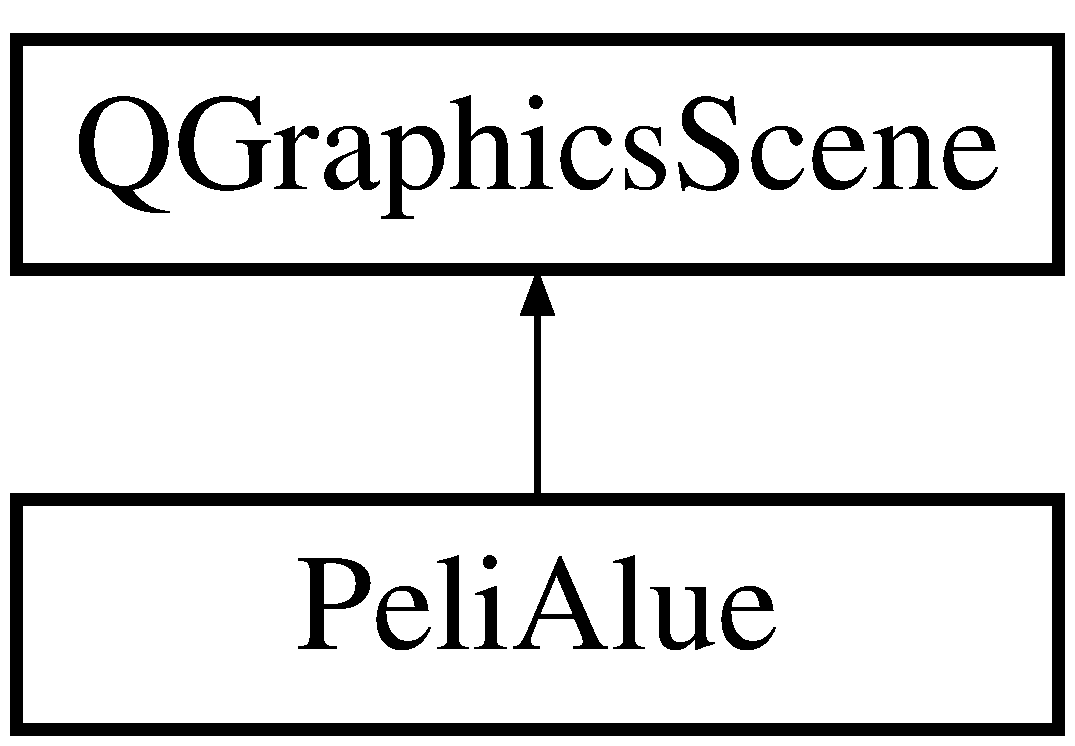
\includegraphics[height=2.000000cm]{class_peli_alue}
\end{center}
\end{figure}
\subsection*{Public Member Functions}
\begin{DoxyCompactItemize}
\item 
void \hyperlink{class_peli_alue_af7359548211f6d9c4b25d40cc8e69270}{lisaa\-Drooni} (\hyperlink{class_drooni}{Drooni} $\ast$drooni)
\begin{DoxyCompactList}\small\item\em lisaa\-Drooni lisää droonin pelialueelle. \end{DoxyCompactList}\end{DoxyCompactItemize}
\subsection*{Protected Member Functions}
\begin{DoxyCompactItemize}
\item 
\hypertarget{class_peli_alue_a21fd493451dbcc935d29a095f57947c4}{void {\bfseries mouse\-Press\-Event} (Q\-Graphics\-Scene\-Mouse\-Event $\ast$mouse\-Event)}\label{class_peli_alue_a21fd493451dbcc935d29a095f57947c4}

\end{DoxyCompactItemize}


\subsection{Member Function Documentation}
\hypertarget{class_peli_alue_af7359548211f6d9c4b25d40cc8e69270}{\index{Peli\-Alue@{Peli\-Alue}!lisaa\-Drooni@{lisaa\-Drooni}}
\index{lisaa\-Drooni@{lisaa\-Drooni}!PeliAlue@{Peli\-Alue}}
\subsubsection[{lisaa\-Drooni}]{\setlength{\rightskip}{0pt plus 5cm}void Peli\-Alue\-::lisaa\-Drooni (
\begin{DoxyParamCaption}
\item[{{\bf Drooni} $\ast$}]{drooni}
\end{DoxyParamCaption}
)}}\label{class_peli_alue_af7359548211f6d9c4b25d40cc8e69270}


lisaa\-Drooni lisää droonin pelialueelle. 


\begin{DoxyParams}{Parameters}
{\em drooni} & Osoitin lisättävään drooniin. \\
\hline
\end{DoxyParams}
\begin{DoxyPrecond}{Precondition}
Pelialueelle ei ole vielä lisätty droonia. 
\end{DoxyPrecond}
\begin{DoxyPostcond}{Postcondition}
\hyperlink{class_drooni}{Drooni} on lisätty pelialueelle. Poikkeustakuu\-: perus 
\end{DoxyPostcond}

\begin{DoxyExceptions}{Exceptions}
{\em Peli\-Virhe} & mikäli pelialueella on jo drooni tai droonin lisäys epäonnistui. \\
\hline
\end{DoxyExceptions}


The documentation for this class was generated from the following files\-:\begin{DoxyCompactItemize}
\item 
\hyperlink{pelialue_8hh}{pelialue.\-hh}\item 
pelialue.\-cpp\end{DoxyCompactItemize}

\hypertarget{class_peli_ikkuna}{\section{Peli\-Ikkuna Class Reference}
\label{class_peli_ikkuna}\index{Peli\-Ikkuna@{Peli\-Ikkuna}}
}
Inheritance diagram for Peli\-Ikkuna\-:\begin{figure}[H]
\begin{center}
\leavevmode
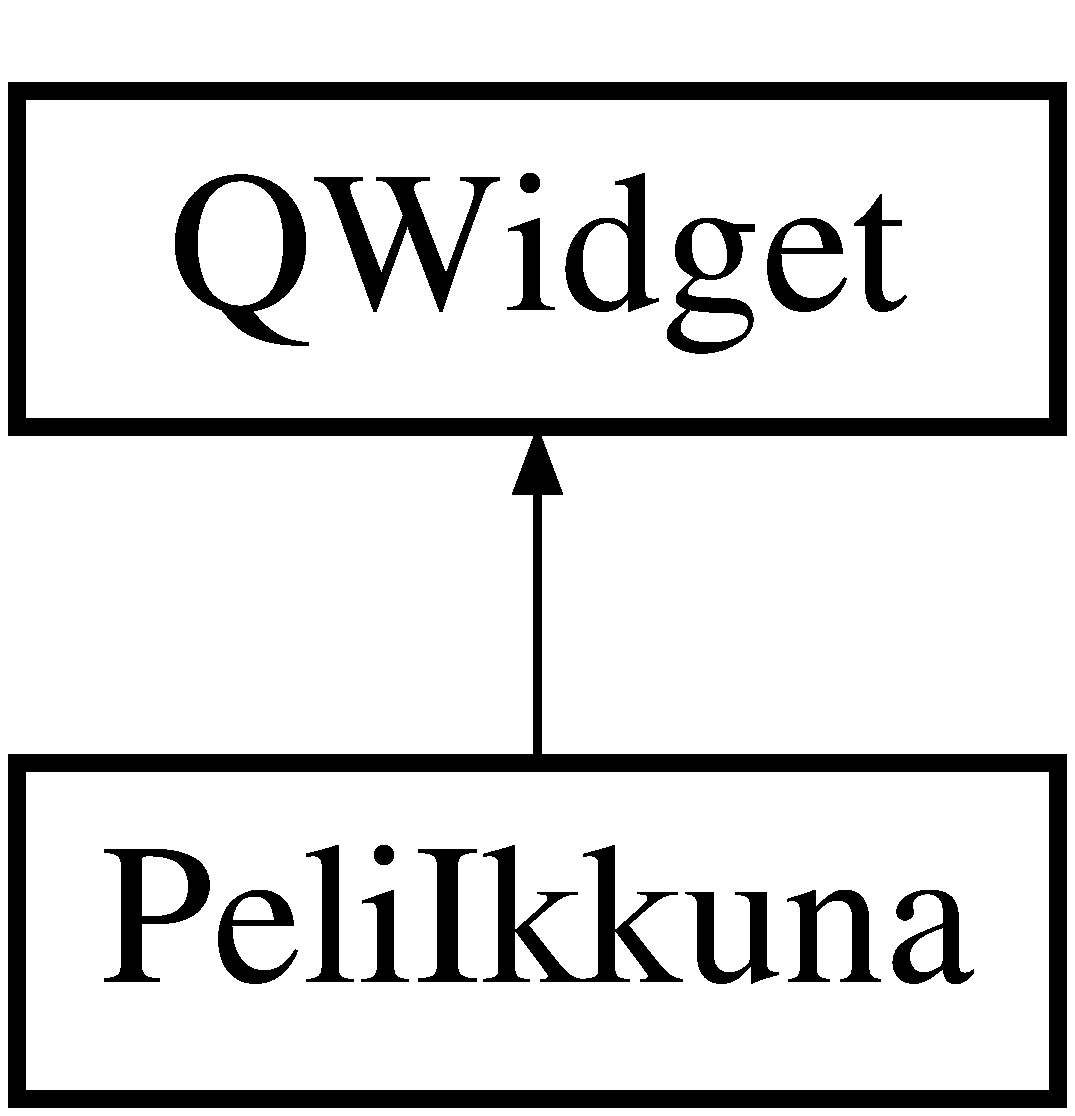
\includegraphics[height=2.000000cm]{class_peli_ikkuna}
\end{center}
\end{figure}
\subsection*{Public Slots}
\begin{DoxyCompactItemize}
\item 
\hypertarget{class_peli_ikkuna_a599ff7ea4e7065407a4cfc376a9e7a4d}{void {\bfseries liikuta\-Viewport} (Q\-Graphics\-Item $\ast$kohde)}\label{class_peli_ikkuna_a599ff7ea4e7065407a4cfc376a9e7a4d}

\item 
\hypertarget{class_peli_ikkuna_a646a8059ff792d36e7dd7c7cc9339945}{void {\bfseries paivita\-Viewport} ()}\label{class_peli_ikkuna_a646a8059ff792d36e7dd7c7cc9339945}

\item 
\hypertarget{class_peli_ikkuna_a14e0c209058d3044db9b782c8b4f4691}{void {\bfseries paivita\-Ammukset} (int ase, int ammuksia)}\label{class_peli_ikkuna_a14e0c209058d3044db9b782c8b4f4691}

\end{DoxyCompactItemize}
\subsection*{Public Member Functions}
\begin{DoxyCompactItemize}
\item 
\hyperlink{class_peli_ikkuna_af57dc5037e1bb4d6056ca9923721ec7d}{Peli\-Ikkuna} (Q\-Widget $\ast$parent=0)
\begin{DoxyCompactList}\small\item\em \hyperlink{class_peli_ikkuna}{Peli\-Ikkuna} luo uuden peli-\/ikkunan. \end{DoxyCompactList}\item 
\hyperlink{class_peli_ikkuna_a185ea9d8d778bace5f12ea619afad966}{$\sim$\-Peli\-Ikkuna} ()
\begin{DoxyCompactList}\small\item\em Peli\-Ikkunan purkaja. \end{DoxyCompactList}\item 
void \hyperlink{class_peli_ikkuna_a42e636f33ca2f6b600a9692eb96c04c0}{aseta\-Kartta} (Q\-Image \&kartta)
\begin{DoxyCompactList}\small\item\em aseta\-Kartta Asettaa pelialueen pohjakartan. \end{DoxyCompactList}\item 
Q\-Graphics\-Pixmap\-Item $\ast$ \hyperlink{class_peli_ikkuna_ace31f5abe08036d2fa3830632f857a7d}{lisaa\-\_\-pysakki} (std\-::shared\-\_\-ptr$<$ Rajapinta\-::\-Pysakki\-R\-P $>$ pysakkiptr)
\begin{DoxyCompactList}\small\item\em lisaa\-\_\-pysakki Lisää pysäkin kartalle \end{DoxyCompactList}\item 
\hyperlink{class_nyssekuva}{Nyssekuva} $\ast$ \hyperlink{class_peli_ikkuna_a3bf868fa2f549d6c3f7fde5ef1e573e0}{lisaa\-\_\-nysse} (std\-::shared\-\_\-ptr$<$ Rajapinta\-::\-Toimija\-R\-P $>$ toimijaptr)
\begin{DoxyCompactList}\small\item\em lisaa\-\_\-nysse Lisää nyssen kartalle \end{DoxyCompactList}\item 
void \hyperlink{class_peli_ikkuna_a6529cb960d0a9c6c1ac809079b6518bc}{lisaa\-Drooni} (\hyperlink{class_drooni}{Drooni} $\ast$drooni)
\begin{DoxyCompactList}\small\item\em lisaa\-Drooni Lisää droonin kartalle. \end{DoxyCompactList}\item 
void \hyperlink{class_peli_ikkuna_aa3943ae9a2c3bd2109deab2b4f9c0c2a}{Paivita\-Tulokset} (std\-::vector$<$ int $>$ tulokset)
\begin{DoxyCompactList}\small\item\em Paivita\-Tulokset Päivittää peliruudulla näytettävät tilastotiedot. \end{DoxyCompactList}\item 
void \hyperlink{class_peli_ikkuna_abee8a20d0f7aa0efbaed03c65238fcab}{nayta\-Toplista} (std\-::vector$<$ Q\-String $>$ huipputulokset)
\begin{DoxyCompactList}\small\item\em nayta\-Toplista Näyttää peliruudulla tämänhetkisen top10 tilanteen. \end{DoxyCompactList}\item 
void \hyperlink{class_peli_ikkuna_a81a7526f0dfedfbd9ca0cfe72331d7d6}{aseta\-Status} (Q\-String status)
\begin{DoxyCompactList}\small\item\em aseta\-Status Asettaa peliruudun statustekstin. \end{DoxyCompactList}\end{DoxyCompactItemize}


\subsection{Constructor \& Destructor Documentation}
\hypertarget{class_peli_ikkuna_af57dc5037e1bb4d6056ca9923721ec7d}{\index{Peli\-Ikkuna@{Peli\-Ikkuna}!Peli\-Ikkuna@{Peli\-Ikkuna}}
\index{Peli\-Ikkuna@{Peli\-Ikkuna}!PeliIkkuna@{Peli\-Ikkuna}}
\subsubsection[{Peli\-Ikkuna}]{\setlength{\rightskip}{0pt plus 5cm}Peli\-Ikkuna\-::\-Peli\-Ikkuna (
\begin{DoxyParamCaption}
\item[{Q\-Widget $\ast$}]{parent = {\ttfamily 0}}
\end{DoxyParamCaption}
)\hspace{0.3cm}{\ttfamily [explicit]}}}\label{class_peli_ikkuna_af57dc5037e1bb4d6056ca9923721ec7d}


\hyperlink{class_peli_ikkuna}{Peli\-Ikkuna} luo uuden peli-\/ikkunan. 


\begin{DoxyParams}{Parameters}
{\em parent} & peli-\/ikkunan vanhempi. Tässä ohjelmassa aina määrittämätön. \\
\hline
\end{DoxyParams}
\begin{DoxyPostcond}{Postcondition}
Ohjelmassa ei ole vielä peli-\/ikkuna oliota. 
\end{DoxyPostcond}
\hypertarget{class_peli_ikkuna_a185ea9d8d778bace5f12ea619afad966}{\index{Peli\-Ikkuna@{Peli\-Ikkuna}!$\sim$\-Peli\-Ikkuna@{$\sim$\-Peli\-Ikkuna}}
\index{$\sim$\-Peli\-Ikkuna@{$\sim$\-Peli\-Ikkuna}!PeliIkkuna@{Peli\-Ikkuna}}
\subsubsection[{$\sim$\-Peli\-Ikkuna}]{\setlength{\rightskip}{0pt plus 5cm}Peli\-Ikkuna\-::$\sim$\-Peli\-Ikkuna (
\begin{DoxyParamCaption}
{}
\end{DoxyParamCaption}
)}}\label{class_peli_ikkuna_a185ea9d8d778bace5f12ea619afad966}


Peli\-Ikkunan purkaja. 

\begin{DoxyPostcond}{Postcondition}
\hyperlink{class_peli_ikkuna}{Peli\-Ikkuna} on poistettu hallitusti. 
\end{DoxyPostcond}


\subsection{Member Function Documentation}
\hypertarget{class_peli_ikkuna_a42e636f33ca2f6b600a9692eb96c04c0}{\index{Peli\-Ikkuna@{Peli\-Ikkuna}!aseta\-Kartta@{aseta\-Kartta}}
\index{aseta\-Kartta@{aseta\-Kartta}!PeliIkkuna@{Peli\-Ikkuna}}
\subsubsection[{aseta\-Kartta}]{\setlength{\rightskip}{0pt plus 5cm}void Peli\-Ikkuna\-::aseta\-Kartta (
\begin{DoxyParamCaption}
\item[{Q\-Image \&}]{kartta}
\end{DoxyParamCaption}
)}}\label{class_peli_ikkuna_a42e636f33ca2f6b600a9692eb96c04c0}


aseta\-Kartta Asettaa pelialueen pohjakartan. 


\begin{DoxyParams}{Parameters}
{\em kartta} & Tampereen keskustan kartta \\
\hline
\end{DoxyParams}
\begin{DoxyPrecond}{Precondition}
Karttaa ei ole vielä asetettu. Kartta on pelilogiikan tarjoama isokartta. 
\end{DoxyPrecond}
\begin{DoxyPostcond}{Postcondition}
Pohjakartta on asetettu. Poikkeustakuu\-: perus 
\end{DoxyPostcond}
\hypertarget{class_peli_ikkuna_a81a7526f0dfedfbd9ca0cfe72331d7d6}{\index{Peli\-Ikkuna@{Peli\-Ikkuna}!aseta\-Status@{aseta\-Status}}
\index{aseta\-Status@{aseta\-Status}!PeliIkkuna@{Peli\-Ikkuna}}
\subsubsection[{aseta\-Status}]{\setlength{\rightskip}{0pt plus 5cm}void Peli\-Ikkuna\-::aseta\-Status (
\begin{DoxyParamCaption}
\item[{Q\-String}]{status}
\end{DoxyParamCaption}
)}}\label{class_peli_ikkuna_a81a7526f0dfedfbd9ca0cfe72331d7d6}


aseta\-Status Asettaa peliruudun statustekstin. 


\begin{DoxyParams}{Parameters}
{\em status} & Haluttu statusteksti \\
\hline
\end{DoxyParams}
\begin{DoxyPrecond}{Precondition}
-\/ 
\end{DoxyPrecond}
\begin{DoxyPostcond}{Postcondition}
Statusteksti on asetettu. Poikkeustakuu\-: perus 
\end{DoxyPostcond}
\hypertarget{class_peli_ikkuna_a3bf868fa2f549d6c3f7fde5ef1e573e0}{\index{Peli\-Ikkuna@{Peli\-Ikkuna}!lisaa\-\_\-nysse@{lisaa\-\_\-nysse}}
\index{lisaa\-\_\-nysse@{lisaa\-\_\-nysse}!PeliIkkuna@{Peli\-Ikkuna}}
\subsubsection[{lisaa\-\_\-nysse}]{\setlength{\rightskip}{0pt plus 5cm}{\bf Nyssekuva} $\ast$ Peli\-Ikkuna\-::lisaa\-\_\-nysse (
\begin{DoxyParamCaption}
\item[{std\-::shared\-\_\-ptr$<$ Rajapinta\-::\-Toimija\-R\-P $>$}]{toimijaptr}
\end{DoxyParamCaption}
)}}\label{class_peli_ikkuna_a3bf868fa2f549d6c3f7fde5ef1e573e0}


lisaa\-\_\-nysse Lisää nyssen kartalle 


\begin{DoxyParams}{Parameters}
{\em toimijaptr} & Osoitin nysseolioon joka toteuttaa Toimija\-R\-P\-:n. \\
\hline
\end{DoxyParams}
\begin{DoxyReturn}{Returns}
Osoitin \hyperlink{class_nyssekuva}{Nyssekuva} olioon. 
\end{DoxyReturn}
\begin{DoxyPrecond}{Precondition}
toimijaptr on nysse ja löytyy kaupungista. 
\end{DoxyPrecond}
\begin{DoxyPostcond}{Postcondition}
Nysse on lisätty onnistuneesti. Poikkeustakuu\-: perus 
\end{DoxyPostcond}
\hypertarget{class_peli_ikkuna_ace31f5abe08036d2fa3830632f857a7d}{\index{Peli\-Ikkuna@{Peli\-Ikkuna}!lisaa\-\_\-pysakki@{lisaa\-\_\-pysakki}}
\index{lisaa\-\_\-pysakki@{lisaa\-\_\-pysakki}!PeliIkkuna@{Peli\-Ikkuna}}
\subsubsection[{lisaa\-\_\-pysakki}]{\setlength{\rightskip}{0pt plus 5cm}Q\-Graphics\-Pixmap\-Item $\ast$ Peli\-Ikkuna\-::lisaa\-\_\-pysakki (
\begin{DoxyParamCaption}
\item[{std\-::shared\-\_\-ptr$<$ Rajapinta\-::\-Pysakki\-R\-P $>$}]{pysakkiptr}
\end{DoxyParamCaption}
)}}\label{class_peli_ikkuna_ace31f5abe08036d2fa3830632f857a7d}


lisaa\-\_\-pysakki Lisää pysäkin kartalle 


\begin{DoxyParams}{Parameters}
{\em pysakkiptr} & Osoitin Pysakki\-R\-P\-:n toteuttavaan pysäkkiolioon \\
\hline
\end{DoxyParams}
\begin{DoxyReturn}{Returns}
Palauttaa osoittimen pysäkkikuva olioon. 
\end{DoxyReturn}
\begin{DoxyPrecond}{Precondition}
Pysäkkiä ei ole vielä piirretty 
\end{DoxyPrecond}
\begin{DoxyPostcond}{Postcondition}
Pysäkki on lisätty onnistuneesti. Poikkeustakuu\-: perus 
\end{DoxyPostcond}
\hypertarget{class_peli_ikkuna_a6529cb960d0a9c6c1ac809079b6518bc}{\index{Peli\-Ikkuna@{Peli\-Ikkuna}!lisaa\-Drooni@{lisaa\-Drooni}}
\index{lisaa\-Drooni@{lisaa\-Drooni}!PeliIkkuna@{Peli\-Ikkuna}}
\subsubsection[{lisaa\-Drooni}]{\setlength{\rightskip}{0pt plus 5cm}void Peli\-Ikkuna\-::lisaa\-Drooni (
\begin{DoxyParamCaption}
\item[{{\bf Drooni} $\ast$}]{drooni}
\end{DoxyParamCaption}
)}}\label{class_peli_ikkuna_a6529cb960d0a9c6c1ac809079b6518bc}


lisaa\-Drooni Lisää droonin kartalle. 


\begin{DoxyParams}{Parameters}
{\em drooni} & Pelissä käytettävä drooniolio \\
\hline
\end{DoxyParams}
\begin{DoxyPrecond}{Precondition}
Droonia ei ole vielä lisätty 
\end{DoxyPrecond}
\begin{DoxyPostcond}{Postcondition}
\hyperlink{class_drooni}{Drooni} on lisätty peliin. Poikkeustakuu\-: perus 
\end{DoxyPostcond}
\hypertarget{class_peli_ikkuna_abee8a20d0f7aa0efbaed03c65238fcab}{\index{Peli\-Ikkuna@{Peli\-Ikkuna}!nayta\-Toplista@{nayta\-Toplista}}
\index{nayta\-Toplista@{nayta\-Toplista}!PeliIkkuna@{Peli\-Ikkuna}}
\subsubsection[{nayta\-Toplista}]{\setlength{\rightskip}{0pt plus 5cm}void Peli\-Ikkuna\-::nayta\-Toplista (
\begin{DoxyParamCaption}
\item[{std\-::vector$<$ Q\-String $>$}]{huipputulokset}
\end{DoxyParamCaption}
)}}\label{class_peli_ikkuna_abee8a20d0f7aa0efbaed03c65238fcab}


nayta\-Toplista Näyttää peliruudulla tämänhetkisen top10 tilanteen. 


\begin{DoxyParams}{Parameters}
{\em huipputulokset} & Vektori top10 tilastosta. \\
\hline
\end{DoxyParams}
\begin{DoxyPrecond}{Precondition}
Top10 listaa ei ole vielä esitetty 
\end{DoxyPrecond}
\begin{DoxyPostcond}{Postcondition}
Top10 lista näkyy peliruudulla. Poikkeustakuu\-: perus 
\end{DoxyPostcond}
\hypertarget{class_peli_ikkuna_aa3943ae9a2c3bd2109deab2b4f9c0c2a}{\index{Peli\-Ikkuna@{Peli\-Ikkuna}!Paivita\-Tulokset@{Paivita\-Tulokset}}
\index{Paivita\-Tulokset@{Paivita\-Tulokset}!PeliIkkuna@{Peli\-Ikkuna}}
\subsubsection[{Paivita\-Tulokset}]{\setlength{\rightskip}{0pt plus 5cm}void Peli\-Ikkuna\-::\-Paivita\-Tulokset (
\begin{DoxyParamCaption}
\item[{std\-::vector$<$ int $>$}]{tulokset}
\end{DoxyParamCaption}
)}}\label{class_peli_ikkuna_aa3943ae9a2c3bd2109deab2b4f9c0c2a}


Paivita\-Tulokset Päivittää peliruudulla näytettävät tilastotiedot. 


\begin{DoxyParams}{Parameters}
{\em tulokset} & Vektori jossa päivitettävät tilastotiedot. \\
\hline
\end{DoxyParams}
\begin{DoxyPrecond}{Precondition}
-\/ 
\end{DoxyPrecond}
\begin{DoxyPostcond}{Postcondition}
Tulokset on päivitetty. Poikkeustakuu\-: perus 
\end{DoxyPostcond}


The documentation for this class was generated from the following files\-:\begin{DoxyCompactItemize}
\item 
\hyperlink{peliikkuna_8hh}{peliikkuna.\-hh}\item 
peliikkuna.\-cpp\end{DoxyCompactItemize}

\hypertarget{class_rynnakkokivaari}{\section{Rynnakkokivaari Class Reference}
\label{class_rynnakkokivaari}\index{Rynnakkokivaari@{Rynnakkokivaari}}
}
Inheritance diagram for Rynnakkokivaari\-:\begin{figure}[H]
\begin{center}
\leavevmode
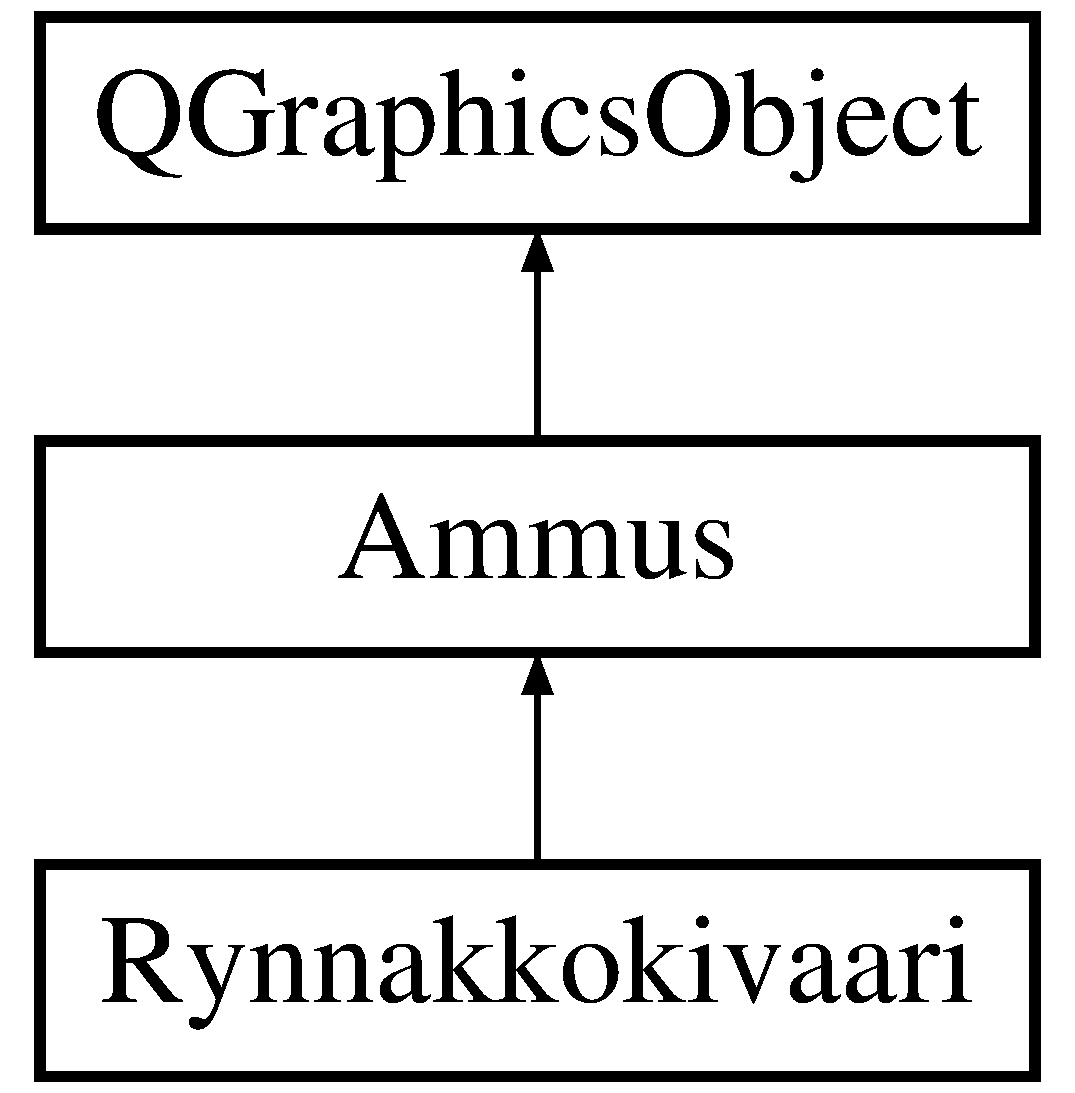
\includegraphics[height=3.000000cm]{class_rynnakkokivaari}
\end{center}
\end{figure}
\subsection*{Public Member Functions}
\begin{DoxyCompactItemize}
\item 
\hyperlink{class_rynnakkokivaari_ad021e0c4cb3b5fb47e98290b279aaec9}{Rynnakkokivaari} (Q\-Graphics\-Item $\ast$parent, qreal suunta)
\begin{DoxyCompactList}\small\item\em Rynnakkokivaarin rakentaja. \end{DoxyCompactList}\item 
\hyperlink{class_rynnakkokivaari_a9f012122077ef373f64c791c89fab206}{$\sim$\-Rynnakkokivaari} ()
\begin{DoxyCompactList}\small\item\em Ammuksen purkaja, tuhoaa new'llä luodun Q\-Timerin. \end{DoxyCompactList}\end{DoxyCompactItemize}
\subsection*{Protected Member Functions}
\begin{DoxyCompactItemize}
\item 
virtual void \hyperlink{class_rynnakkokivaari_a3b09e5434760dd51d7aeb5834520e52d}{aseta\-Ammuskuva} ()
\begin{DoxyCompactList}\small\item\em aseta\-Ammuskuva asettaa ammuksen ulkoasun. Toteutettava periytetyssä luokassa, asetettava ammuskuva on Q\-Image Ammus\-::ammuskuva. \end{DoxyCompactList}\end{DoxyCompactItemize}
\subsection*{Additional Inherited Members}


\subsection{Constructor \& Destructor Documentation}
\hypertarget{class_rynnakkokivaari_ad021e0c4cb3b5fb47e98290b279aaec9}{\index{Rynnakkokivaari@{Rynnakkokivaari}!Rynnakkokivaari@{Rynnakkokivaari}}
\index{Rynnakkokivaari@{Rynnakkokivaari}!Rynnakkokivaari@{Rynnakkokivaari}}
\subsubsection[{Rynnakkokivaari}]{\setlength{\rightskip}{0pt plus 5cm}Rynnakkokivaari\-::\-Rynnakkokivaari (
\begin{DoxyParamCaption}
\item[{Q\-Graphics\-Item $\ast$}]{parent, }
\item[{qreal}]{suunta}
\end{DoxyParamCaption}
)}}\label{class_rynnakkokivaari_ad021e0c4cb3b5fb47e98290b279aaec9}


Rynnakkokivaarin rakentaja. 


\begin{DoxyParams}{Parameters}
{\em parent} & ammuksen ampuja \\
\hline
{\em suunta} & ammuksen lähtösuunta \\
\hline
\end{DoxyParams}
\begin{DoxyPostcond}{Postcondition}
Rynnäkkökiväärin ammus on alustettu ja toiminnassa. Poikkeustakuu\-: perus 
\end{DoxyPostcond}
\hypertarget{class_rynnakkokivaari_a9f012122077ef373f64c791c89fab206}{\index{Rynnakkokivaari@{Rynnakkokivaari}!$\sim$\-Rynnakkokivaari@{$\sim$\-Rynnakkokivaari}}
\index{$\sim$\-Rynnakkokivaari@{$\sim$\-Rynnakkokivaari}!Rynnakkokivaari@{Rynnakkokivaari}}
\subsubsection[{$\sim$\-Rynnakkokivaari}]{\setlength{\rightskip}{0pt plus 5cm}Rynnakkokivaari\-::$\sim$\-Rynnakkokivaari (
\begin{DoxyParamCaption}
{}
\end{DoxyParamCaption}
)}}\label{class_rynnakkokivaari_a9f012122077ef373f64c791c89fab206}


Ammuksen purkaja, tuhoaa new'llä luodun Q\-Timerin. 

\begin{DoxyPostcond}{Postcondition}
ammus on tuhottu oikein. 
\end{DoxyPostcond}


\subsection{Member Function Documentation}
\hypertarget{class_rynnakkokivaari_a3b09e5434760dd51d7aeb5834520e52d}{\index{Rynnakkokivaari@{Rynnakkokivaari}!aseta\-Ammuskuva@{aseta\-Ammuskuva}}
\index{aseta\-Ammuskuva@{aseta\-Ammuskuva}!Rynnakkokivaari@{Rynnakkokivaari}}
\subsubsection[{aseta\-Ammuskuva}]{\setlength{\rightskip}{0pt plus 5cm}void Rynnakkokivaari\-::aseta\-Ammuskuva (
\begin{DoxyParamCaption}
{}
\end{DoxyParamCaption}
)\hspace{0.3cm}{\ttfamily [protected]}, {\ttfamily [virtual]}}}\label{class_rynnakkokivaari_a3b09e5434760dd51d7aeb5834520e52d}


aseta\-Ammuskuva asettaa ammuksen ulkoasun. Toteutettava periytetyssä luokassa, asetettava ammuskuva on Q\-Image Ammus\-::ammuskuva. 

\begin{DoxyPrecond}{Precondition}
-\/ 
\end{DoxyPrecond}
\begin{DoxyPostcond}{Postcondition}
Ammus\-::ammuskuva on asetettu. Poikkeustakuu\-: perus 
\end{DoxyPostcond}

\begin{DoxyExceptions}{Exceptions}
{\em Peli\-Virhe} & Ammuskuvan avaaminen epäonnistui. \\
\hline
\end{DoxyExceptions}


Implements \hyperlink{class_ammus_a637789fc7748679d5e6ceeb7bb2d24a4}{Ammus}.



The documentation for this class was generated from the following files\-:\begin{DoxyCompactItemize}
\item 
\hyperlink{rynnakkokivaari_8hh}{rynnakkokivaari.\-hh}\item 
rynnakkokivaari.\-cpp\end{DoxyCompactItemize}

\hypertarget{class_tilasto}{\section{Tilasto Class Reference}
\label{class_tilasto}\index{Tilasto@{Tilasto}}
}
Inheritance diagram for Tilasto\-:\begin{figure}[H]
\begin{center}
\leavevmode
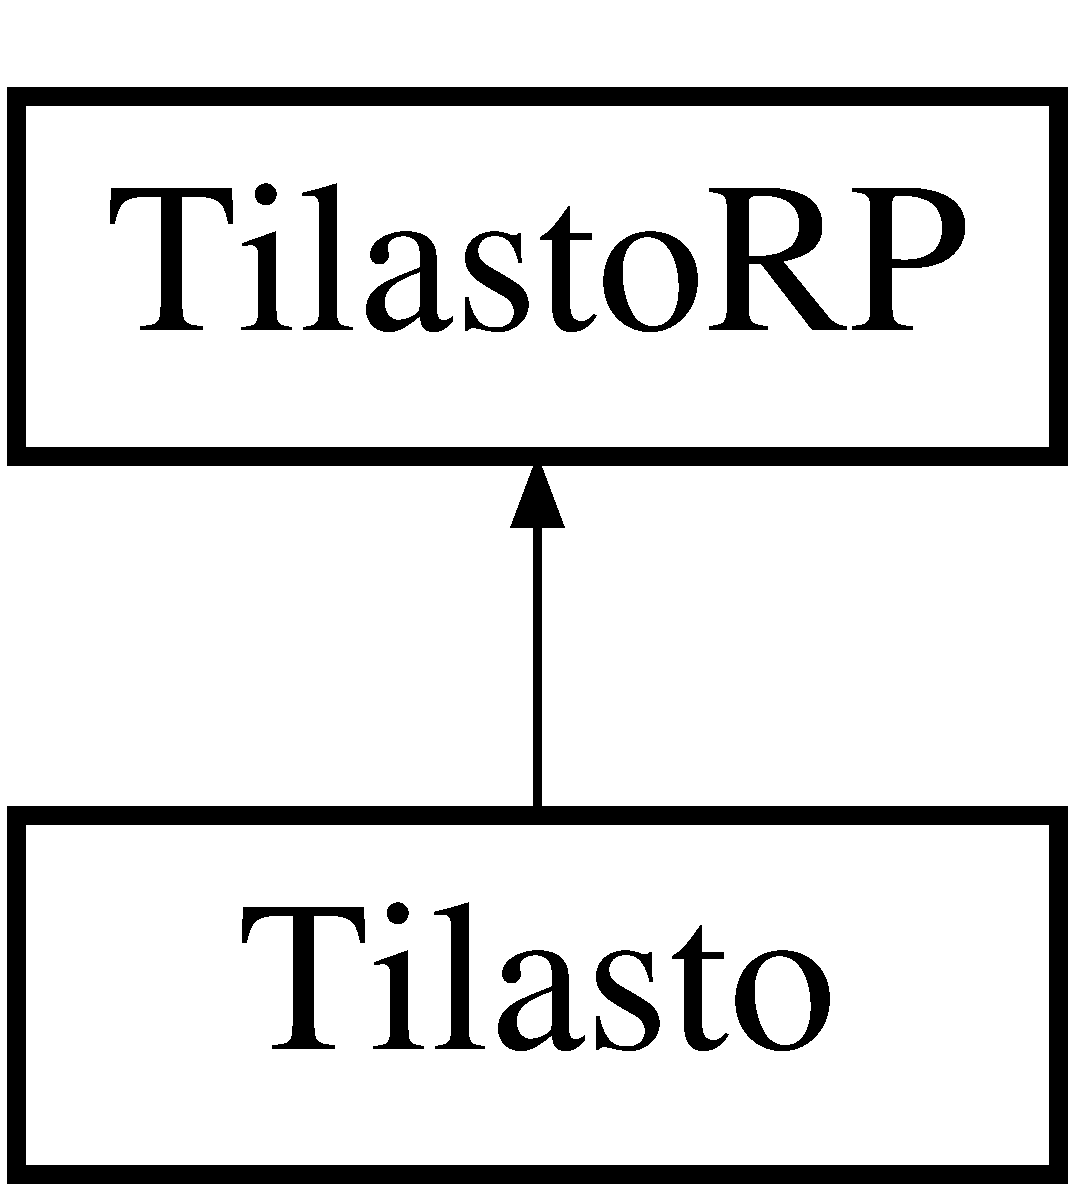
\includegraphics[height=2.000000cm]{class_tilasto}
\end{center}
\end{figure}
\subsection*{Public Member Functions}
\begin{DoxyCompactItemize}
\item 
\hypertarget{class_tilasto_ae9dc95097a968eec3e7ccf95802ca1ad}{virtual int {\bfseries anna\-Pisteet} () const }\label{class_tilasto_ae9dc95097a968eec3e7ccf95802ca1ad}

\item 
\hypertarget{class_tilasto_aee07b758b26e74787301d885134072cd}{virtual void {\bfseries matkustajia\-Kuoli} (int lkm)}\label{class_tilasto_aee07b758b26e74787301d885134072cd}

\item 
\hypertarget{class_tilasto_acc175adaef0890e7a619ffb647d1b712}{virtual void {\bfseries lisaa\-Matkustajia} (int lkm)}\label{class_tilasto_acc175adaef0890e7a619ffb647d1b712}

\item 
\hypertarget{class_tilasto_a9b424d80452e7c7e30e2ec3b2b67202c}{virtual void {\bfseries nysse\-Tuhoutui} ()}\label{class_tilasto_a9b424d80452e7c7e30e2ec3b2b67202c}

\item 
\hypertarget{class_tilasto_a02eeb0e7cadc5364bf6775923a538f28}{virtual void {\bfseries uusi\-Nysse} ()}\label{class_tilasto_a02eeb0e7cadc5364bf6775923a538f28}

\item 
\hypertarget{class_tilasto_ad1f3fdb38673138ef2472ada5a7a1400}{virtual void {\bfseries nysse\-Poistui} ()}\label{class_tilasto_ad1f3fdb38673138ef2472ada5a7a1400}

\item 
std\-::vector$<$ int $>$ \hyperlink{class_tilasto_a3d52332ec15d3cfb8a328ca5706ca7ab}{paivita\-\_\-tilasto} () const 
\begin{DoxyCompactList}\small\item\em paivita\-\_\-tilasto palauttaa kaupungille pistetaulua varten tarvittavat luvut. \end{DoxyCompactList}\item 
std\-::vector$<$ Q\-String $>$ \hyperlink{class_tilasto_a86702f1421079639ef7cd6d9a8c24019}{lue\-\_\-tiedosto} (Q\-String)
\begin{DoxyCompactList}\small\item\em lue\-\_\-tiedosto lukee tekstitiedoston, johon on tallennettu parhaiden pelaajien tiedot \end{DoxyCompactList}\item 
void \hyperlink{class_tilasto_a884916e254892439f8f4e8e3fa144566}{kirjoita\-Tiedostoon} (int, Q\-String) const 
\begin{DoxyCompactList}\small\item\em kirjoita\-Tiedostoon lisää pelaajan tuloksen top-\/listalle, jos on aihetta \end{DoxyCompactList}\item 
int \hyperlink{class_tilasto_a76f09fa3ec7ca9031b0143bcac01b882}{selvita\-Listasijoitus} (int uusi\-Tulos) const 
\begin{DoxyCompactList}\small\item\em selvita\-Listasijoitus Kertoo sijoituksen top 10 listalla annetuilla pisteillä. \end{DoxyCompactList}\end{DoxyCompactItemize}


\subsection{Member Function Documentation}
\hypertarget{class_tilasto_a884916e254892439f8f4e8e3fa144566}{\index{Tilasto@{Tilasto}!kirjoita\-Tiedostoon@{kirjoita\-Tiedostoon}}
\index{kirjoita\-Tiedostoon@{kirjoita\-Tiedostoon}!Tilasto@{Tilasto}}
\subsubsection[{kirjoita\-Tiedostoon}]{\setlength{\rightskip}{0pt plus 5cm}void Tilasto\-::kirjoita\-Tiedostoon (
\begin{DoxyParamCaption}
\item[{int}]{tulos, }
\item[{Q\-String}]{nimi}
\end{DoxyParamCaption}
) const}}\label{class_tilasto_a884916e254892439f8f4e8e3fa144566}


kirjoita\-Tiedostoon lisää pelaajan tuloksen top-\/listalle, jos on aihetta 


\begin{DoxyParams}{Parameters}
{\em pelaajan} & tulos ja nimi \\
\hline
\end{DoxyParams}
\begin{DoxyPrecond}{Precondition}
tiedosto johon kirjoitetaan on olemassa 
\end{DoxyPrecond}
\begin{DoxyPostcond}{Postcondition}
poikkeustakuu\-: vahva 
\end{DoxyPostcond}
\hypertarget{class_tilasto_a86702f1421079639ef7cd6d9a8c24019}{\index{Tilasto@{Tilasto}!lue\-\_\-tiedosto@{lue\-\_\-tiedosto}}
\index{lue\-\_\-tiedosto@{lue\-\_\-tiedosto}!Tilasto@{Tilasto}}
\subsubsection[{lue\-\_\-tiedosto}]{\setlength{\rightskip}{0pt plus 5cm}std\-::vector$<$ Q\-String $>$ Tilasto\-::lue\-\_\-tiedosto (
\begin{DoxyParamCaption}
\item[{Q\-String}]{tiedosto}
\end{DoxyParamCaption}
)}}\label{class_tilasto_a86702f1421079639ef7cd6d9a8c24019}


lue\-\_\-tiedosto lukee tekstitiedoston, johon on tallennettu parhaiden pelaajien tiedot 

\begin{DoxyReturn}{Returns}
vektorin, jossa alkioina on tiedoston rivi tallenettuna Q\-Stringiin 
\end{DoxyReturn}
\begin{DoxyPrecond}{Precondition}
tiedoston rivit on muotoa \char`\"{} nimi tulos \char`\"{} 
\end{DoxyPrecond}
\begin{DoxyPostcond}{Postcondition}
poikkeustakuu\-: vahva 
\end{DoxyPostcond}

\begin{DoxyParams}{Parameters}
{\em tiedoston} & hakupolku \\
\hline
\end{DoxyParams}
\hypertarget{class_tilasto_a3d52332ec15d3cfb8a328ca5706ca7ab}{\index{Tilasto@{Tilasto}!paivita\-\_\-tilasto@{paivita\-\_\-tilasto}}
\index{paivita\-\_\-tilasto@{paivita\-\_\-tilasto}!Tilasto@{Tilasto}}
\subsubsection[{paivita\-\_\-tilasto}]{\setlength{\rightskip}{0pt plus 5cm}std\-::vector$<$ int $>$ Tilasto\-::paivita\-\_\-tilasto (
\begin{DoxyParamCaption}
{}
\end{DoxyParamCaption}
) const}}\label{class_tilasto_a3d52332ec15d3cfb8a328ca5706ca7ab}


paivita\-\_\-tilasto palauttaa kaupungille pistetaulua varten tarvittavat luvut. 

\begin{DoxyReturn}{Returns}
vektori, jossa on 5 tilaston private muuttujaa 
\end{DoxyReturn}
\begin{DoxyPrecond}{Precondition}
olio rakennettu 
\end{DoxyPrecond}
\begin{DoxyPostcond}{Postcondition}
poikkeustakuu\-: vahva 
\end{DoxyPostcond}
\hypertarget{class_tilasto_a76f09fa3ec7ca9031b0143bcac01b882}{\index{Tilasto@{Tilasto}!selvita\-Listasijoitus@{selvita\-Listasijoitus}}
\index{selvita\-Listasijoitus@{selvita\-Listasijoitus}!Tilasto@{Tilasto}}
\subsubsection[{selvita\-Listasijoitus}]{\setlength{\rightskip}{0pt plus 5cm}int Tilasto\-::selvita\-Listasijoitus (
\begin{DoxyParamCaption}
\item[{int}]{uusi\-Tulos}
\end{DoxyParamCaption}
) const}}\label{class_tilasto_a76f09fa3ec7ca9031b0143bcac01b882}


selvita\-Listasijoitus Kertoo sijoituksen top 10 listalla annetuilla pisteillä. 


\begin{DoxyParams}{Parameters}
{\em uusi\-Tulos} & Pisteet joidenka sijoitus halutaan. \\
\hline
\end{DoxyParams}
\begin{DoxyReturn}{Returns}
Sijoitus top10 listalla, 11 jos ei top10 listalla 
\end{DoxyReturn}
\begin{DoxyPrecond}{Precondition}
-\/ 
\end{DoxyPrecond}
\begin{DoxyPostcond}{Postcondition}
Poikkeustakuu\-: vahva 
\end{DoxyPostcond}


The documentation for this class was generated from the following files\-:\begin{DoxyCompactItemize}
\item 
tilasto.\-hh\item 
tilasto.\-cpp\end{DoxyCompactItemize}

\chapter{File Documentation}
\hypertarget{ammus_8hh}{\section{ammus.\-hh File Reference}
\label{ammus_8hh}\index{ammus.\-hh@{ammus.\-hh}}
}


Kantaluokka kaikille pelissä käytettäville ammuksille. Tarjoaa perustoiminnoille toteutukset. Muistin loppuessa heittää std\-::bad\-\_\-alloc ellei poikkeustakuu ole nothrow.  


{\ttfamily \#include $<$Q\-Graphics\-Object$>$}\\*
{\ttfamily \#include $<$Q\-Timer$>$}\\*
{\ttfamily \#include $<$Q\-Point\-F$>$}\\*
\subsection*{Classes}
\begin{DoxyCompactItemize}
\item 
class \hyperlink{class_ammus}{Ammus}
\end{DoxyCompactItemize}


\subsection{Detailed Description}
Kantaluokka kaikille pelissä käytettäville ammuksille. Tarjoaa perustoiminnoille toteutukset. Muistin loppuessa heittää std\-::bad\-\_\-alloc ellei poikkeustakuu ole nothrow. 
\hypertarget{drooni_8hh}{\section{drooni.\-hh File Reference}
\label{drooni_8hh}\index{drooni.\-hh@{drooni.\-hh}}
}


\hyperlink{class_drooni}{Drooni} luokka toteuttaa pelissä käytettävän droonin. Periytetty Q\-Graphics\-Object ja Toimija\-R\-P luokista.  


{\ttfamily \#include \char`\"{}toimijarp.\-hh\char`\"{}}\\*
{\ttfamily \#include \char`\"{}sijainti.\-hh\char`\"{}}\\*
{\ttfamily \#include \char`\"{}rynnakkokivaari.\-hh\char`\"{}}\\*
{\ttfamily \#include $<$Q\-Graphics\-Object$>$}\\*
{\ttfamily \#include $<$Q\-Image$>$}\\*
{\ttfamily \#include $<$Q\-Point\-F$>$}\\*
{\ttfamily \#include $<$Q\-Timer$>$}\\*
\subsection*{Classes}
\begin{DoxyCompactItemize}
\item 
class \hyperlink{class_drooni}{Drooni}
\end{DoxyCompactItemize}


\subsection{Detailed Description}
\hyperlink{class_drooni}{Drooni} luokka toteuttaa pelissä käytettävän droonin. Periytetty Q\-Graphics\-Object ja Toimija\-R\-P luokista. 
\hypertarget{kaupunki_8hh}{\section{kaupunki.\-hh File Reference}
\label{kaupunki_8hh}\index{kaupunki.\-hh@{kaupunki.\-hh}}
}


\hyperlink{class_kaupunki}{Kaupunki} luokka on Kaupunki\-R\-P\-:stä periytetty. \hyperlink{class_kaupunki}{Kaupunki} hallinnoi pelin tapahtumia.  


{\ttfamily \#include \char`\"{}kaupunkirp.\-hh\char`\"{}}\\*
{\ttfamily \#include \char`\"{}pysakkirp.\-hh\char`\"{}}\\*
{\ttfamily \#include \char`\"{}toimijarp.\-hh\char`\"{}}\\*
{\ttfamily \#include \char`\"{}peliikkuna.\-hh\char`\"{}}\\*
{\ttfamily \#include \char`\"{}drooni.\-hh\char`\"{}}\\*
{\ttfamily \#include \char`\"{}tilasto.\-hh\char`\"{}}\\*
{\ttfamily \#include \char`\"{}nyssekuva.\-hh\char`\"{}}\\*
{\ttfamily \#include $<$memory$>$}\\*
{\ttfamily \#include $<$vector$>$}\\*
{\ttfamily \#include $<$unordered\-\_\-map$>$}\\*
{\ttfamily \#include $<$Q\-Image$>$}\\*
{\ttfamily \#include $<$Q\-Time$>$}\\*
{\ttfamily \#include $<$Q\-Graphics\-Object$>$}\\*
{\ttfamily \#include $<$Q\-Object$>$}\\*
\subsection*{Classes}
\begin{DoxyCompactItemize}
\item 
class \hyperlink{class_kaupunki}{Kaupunki}
\end{DoxyCompactItemize}


\subsection{Detailed Description}
\hyperlink{class_kaupunki}{Kaupunki} luokka on Kaupunki\-R\-P\-:stä periytetty. \hyperlink{class_kaupunki}{Kaupunki} hallinnoi pelin tapahtumia. 
\hypertarget{laser_8hh}{\section{laser.\-hh File Reference}
\label{laser_8hh}\index{laser.\-hh@{laser.\-hh}}
}


\hyperlink{class_ammus}{Ammus} luokasta periytetty luokka, määrittelee laserin toiminnan.  


{\ttfamily \#include \char`\"{}ammus.\-hh\char`\"{}}\\*
{\ttfamily \#include $<$Q\-Graphics\-Object$>$}\\*
{\ttfamily \#include $<$Q\-Rect\-F$>$}\\*
\subsection*{Classes}
\begin{DoxyCompactItemize}
\item 
class \hyperlink{class_laser}{Laser}
\end{DoxyCompactItemize}


\subsection{Detailed Description}
\hyperlink{class_ammus}{Ammus} luokasta periytetty luokka, määrittelee laserin toiminnan. 
\hypertarget{miina_8hh}{\section{miina.\-hh File Reference}
\label{miina_8hh}\index{miina.\-hh@{miina.\-hh}}
}


\hyperlink{class_ammus}{Ammus} luokasta periytetty luokka, määrittelee miinan toiminnan. Räjähdyksessä käytetyt kuvat \href{http://wrathgames.com/blog}{\tt http\-://wrathgames.\-com/blog} Wrath\-Games Studio. Muistin loppuessa voidaan heittää aina std\-::bad\-\_\-alloc.  


{\ttfamily \#include \char`\"{}ammus.\-hh\char`\"{}}\\*
{\ttfamily \#include $<$Q\-Graphics\-Object$>$}\\*
{\ttfamily \#include $<$Q\-Point\-F$>$}\\*
{\ttfamily \#include $<$unordered\-\_\-map$>$}\\*
{\ttfamily \#include $<$Q\-Image$>$}\\*
{\ttfamily \#include $<$Q\-Property\-Animation$>$}\\*
\subsection*{Classes}
\begin{DoxyCompactItemize}
\item 
class \hyperlink{class_miina}{Miina}
\end{DoxyCompactItemize}


\subsection{Detailed Description}
\hyperlink{class_ammus}{Ammus} luokasta periytetty luokka, määrittelee miinan toiminnan. Räjähdyksessä käytetyt kuvat \href{http://wrathgames.com/blog}{\tt http\-://wrathgames.\-com/blog} Wrath\-Games Studio. Muistin loppuessa voidaan heittää aina std\-::bad\-\_\-alloc. 
\hypertarget{nyssekuva_8hh}{\section{nyssekuva.\-hh File Reference}
\label{nyssekuva_8hh}\index{nyssekuva.\-hh@{nyssekuva.\-hh}}
}


\hyperlink{class_nyssekuva}{Nyssekuva} tarjoaa graafisen ilmeen pelin nysseille. Periytetty Q\-Graphics\-Itemista.  


{\ttfamily \#include \char`\"{}kaupunkirp.\-hh\char`\"{}}\\*
{\ttfamily \#include $<$toimijarp.\-hh$>$}\\*
{\ttfamily \#include $<$Q\-Graphics\-Pixmap\-Item$>$}\\*
{\ttfamily \#include $<$Q\-Pixmap$>$}\\*
{\ttfamily \#include $<$Q\-Graphics\-Item$>$}\\*
{\ttfamily \#include $<$memory$>$}\\*
\subsection*{Classes}
\begin{DoxyCompactItemize}
\item 
class \hyperlink{class_nyssekuva}{Nyssekuva}
\end{DoxyCompactItemize}


\subsection{Detailed Description}
\hyperlink{class_nyssekuva}{Nyssekuva} tarjoaa graafisen ilmeen pelin nysseille. Periytetty Q\-Graphics\-Itemista. 
\hypertarget{pelialue_8hh}{\section{pelialue.\-hh File Reference}
\label{pelialue_8hh}\index{pelialue.\-hh@{pelialue.\-hh}}
}


\hyperlink{class_peli_alue}{Peli\-Alue} on periytetty Q\-Graphics\-Scenestä pelin tarkoituksiin sopivaksi.  


{\ttfamily \#include \char`\"{}drooni.\-hh\char`\"{}}\\*
{\ttfamily \#include $<$Q\-Graphics\-Scene$>$}\\*
{\ttfamily \#include $<$Q\-Graphics\-Scene\-Mouse\-Event$>$}\\*
\subsection*{Classes}
\begin{DoxyCompactItemize}
\item 
class \hyperlink{class_peli_alue}{Peli\-Alue}
\end{DoxyCompactItemize}


\subsection{Detailed Description}
\hyperlink{class_peli_alue}{Peli\-Alue} on periytetty Q\-Graphics\-Scenestä pelin tarkoituksiin sopivaksi. 
\hypertarget{peliikkuna_8hh}{\section{peliikkuna.\-hh File Reference}
\label{peliikkuna_8hh}\index{peliikkuna.\-hh@{peliikkuna.\-hh}}
}


\hyperlink{class_peli_ikkuna}{Peli\-Ikkuna} on pelin \char`\"{}pääikkunan\char`\"{} tarjoava luokka.  


{\ttfamily \#include \char`\"{}pysakkirp.\-hh\char`\"{}}\\*
{\ttfamily \#include \char`\"{}nyssekuva.\-hh\char`\"{}}\\*
{\ttfamily \#include \char`\"{}pelialue.\-hh\char`\"{}}\\*
{\ttfamily \#include \char`\"{}drooni.\-hh\char`\"{}}\\*
{\ttfamily \#include $<$Q\-Widget$>$}\\*
{\ttfamily \#include $<$Q\-Image$>$}\\*
{\ttfamily \#include $<$Q\-Graphics\-Scene$>$}\\*
{\ttfamily \#include $<$Q\-Graphics\-Item$>$}\\*
{\ttfamily \#include $<$Q\-Graphics\-Pixmap\-Item$>$}\\*
{\ttfamily \#include $<$Q\-Point\-F$>$}\\*
{\ttfamily \#include $<$Q\-String$>$}\\*
{\ttfamily \#include $<$Q\-Timer$>$}\\*
{\ttfamily \#include $<$vector$>$}\\*
\subsection*{Classes}
\begin{DoxyCompactItemize}
\item 
class \hyperlink{class_peli_ikkuna}{Peli\-Ikkuna}
\end{DoxyCompactItemize}


\subsection{Detailed Description}
\hyperlink{class_peli_ikkuna}{Peli\-Ikkuna} on pelin \char`\"{}pääikkunan\char`\"{} tarjoava luokka. 
\hypertarget{rynnakkokivaari_8hh}{\section{rynnakkokivaari.\-hh File Reference}
\label{rynnakkokivaari_8hh}\index{rynnakkokivaari.\-hh@{rynnakkokivaari.\-hh}}
}


\hyperlink{class_ammus}{Ammus} luokasta periytetty luokka, määrittelee rynnäkkökiväärin ammuksen.  


{\ttfamily \#include \char`\"{}ammus.\-hh\char`\"{}}\\*
{\ttfamily \#include $<$Q\-Graphics\-Object$>$}\\*
{\ttfamily \#include $<$Q\-Point\-F$>$}\\*
\subsection*{Classes}
\begin{DoxyCompactItemize}
\item 
class \hyperlink{class_rynnakkokivaari}{Rynnakkokivaari}
\end{DoxyCompactItemize}


\subsection{Detailed Description}
\hyperlink{class_ammus}{Ammus} luokasta periytetty luokka, määrittelee rynnäkkökiväärin ammuksen. 
%--- End generated contents ---

% Index
\newpage
\phantomsection
\addcontentsline{toc}{part}{Index}
\printindex

\end{document}
